\documentclass[10pt,]{article}
\usepackage[]{mathpazo}
\usepackage{amssymb,amsmath}
\usepackage{ifxetex,ifluatex}
\usepackage{fixltx2e} % provides \textsubscript
\ifnum 0\ifxetex 1\fi\ifluatex 1\fi=0 % if pdftex
  \usepackage[T1]{fontenc}
  \usepackage[utf8]{inputenc}
\else % if luatex or xelatex
  \ifxetex
    \usepackage{mathspec}
  \else
    \usepackage{fontspec}
  \fi
  \defaultfontfeatures{Ligatures=TeX,Scale=MatchLowercase}
\fi
% use upquote if available, for straight quotes in verbatim environments
\IfFileExists{upquote.sty}{\usepackage{upquote}}{}
% use microtype if available
\IfFileExists{microtype.sty}{%
\usepackage{microtype}
\UseMicrotypeSet[protrusion]{basicmath} % disable protrusion for tt fonts
}{}
\usepackage[margin=0.75in]{geometry}
\usepackage{hyperref}
\hypersetup{unicode=true,
            pdftitle={Summary of Trade and Tariff Data, Quantity Gap},
            pdfborder={0 0 0},
            breaklinks=true}
\urlstyle{same}  % don't use monospace font for urls
\usepackage{natbib}
\bibliographystyle{plainnat}
\usepackage{color}
\usepackage{fancyvrb}
\newcommand{\VerbBar}{|}
\newcommand{\VERB}{\Verb[commandchars=\\\{\}]}
\DefineVerbatimEnvironment{Highlighting}{Verbatim}{commandchars=\\\{\}}
% Add ',fontsize=\small' for more characters per line
\usepackage{framed}
\definecolor{shadecolor}{RGB}{248,248,248}
\newenvironment{Shaded}{\begin{snugshade}}{\end{snugshade}}
\newcommand{\KeywordTok}[1]{\textcolor[rgb]{0.13,0.29,0.53}{\textbf{{#1}}}}
\newcommand{\DataTypeTok}[1]{\textcolor[rgb]{0.13,0.29,0.53}{{#1}}}
\newcommand{\DecValTok}[1]{\textcolor[rgb]{0.00,0.00,0.81}{{#1}}}
\newcommand{\BaseNTok}[1]{\textcolor[rgb]{0.00,0.00,0.81}{{#1}}}
\newcommand{\FloatTok}[1]{\textcolor[rgb]{0.00,0.00,0.81}{{#1}}}
\newcommand{\ConstantTok}[1]{\textcolor[rgb]{0.00,0.00,0.00}{{#1}}}
\newcommand{\CharTok}[1]{\textcolor[rgb]{0.31,0.60,0.02}{{#1}}}
\newcommand{\SpecialCharTok}[1]{\textcolor[rgb]{0.00,0.00,0.00}{{#1}}}
\newcommand{\StringTok}[1]{\textcolor[rgb]{0.31,0.60,0.02}{{#1}}}
\newcommand{\VerbatimStringTok}[1]{\textcolor[rgb]{0.31,0.60,0.02}{{#1}}}
\newcommand{\SpecialStringTok}[1]{\textcolor[rgb]{0.31,0.60,0.02}{{#1}}}
\newcommand{\ImportTok}[1]{{#1}}
\newcommand{\CommentTok}[1]{\textcolor[rgb]{0.56,0.35,0.01}{\textit{{#1}}}}
\newcommand{\DocumentationTok}[1]{\textcolor[rgb]{0.56,0.35,0.01}{\textbf{\textit{{#1}}}}}
\newcommand{\AnnotationTok}[1]{\textcolor[rgb]{0.56,0.35,0.01}{\textbf{\textit{{#1}}}}}
\newcommand{\CommentVarTok}[1]{\textcolor[rgb]{0.56,0.35,0.01}{\textbf{\textit{{#1}}}}}
\newcommand{\OtherTok}[1]{\textcolor[rgb]{0.56,0.35,0.01}{{#1}}}
\newcommand{\FunctionTok}[1]{\textcolor[rgb]{0.00,0.00,0.00}{{#1}}}
\newcommand{\VariableTok}[1]{\textcolor[rgb]{0.00,0.00,0.00}{{#1}}}
\newcommand{\ControlFlowTok}[1]{\textcolor[rgb]{0.13,0.29,0.53}{\textbf{{#1}}}}
\newcommand{\OperatorTok}[1]{\textcolor[rgb]{0.81,0.36,0.00}{\textbf{{#1}}}}
\newcommand{\BuiltInTok}[1]{{#1}}
\newcommand{\ExtensionTok}[1]{{#1}}
\newcommand{\PreprocessorTok}[1]{\textcolor[rgb]{0.56,0.35,0.01}{\textit{{#1}}}}
\newcommand{\AttributeTok}[1]{\textcolor[rgb]{0.77,0.63,0.00}{{#1}}}
\newcommand{\RegionMarkerTok}[1]{{#1}}
\newcommand{\InformationTok}[1]{\textcolor[rgb]{0.56,0.35,0.01}{\textbf{\textit{{#1}}}}}
\newcommand{\WarningTok}[1]{\textcolor[rgb]{0.56,0.35,0.01}{\textbf{\textit{{#1}}}}}
\newcommand{\AlertTok}[1]{\textcolor[rgb]{0.94,0.16,0.16}{{#1}}}
\newcommand{\ErrorTok}[1]{\textcolor[rgb]{0.64,0.00,0.00}{\textbf{{#1}}}}
\newcommand{\NormalTok}[1]{{#1}}
\usepackage{longtable,booktabs}
\usepackage{graphicx,grffile}
\makeatletter
\def\maxwidth{\ifdim\Gin@nat@width>\linewidth\linewidth\else\Gin@nat@width\fi}
\def\maxheight{\ifdim\Gin@nat@height>\textheight\textheight\else\Gin@nat@height\fi}
\makeatother
% Scale images if necessary, so that they will not overflow the page
% margins by default, and it is still possible to overwrite the defaults
% using explicit options in \includegraphics[width, height, ...]{}
\setkeys{Gin}{width=\maxwidth,height=\maxheight,keepaspectratio}
\IfFileExists{parskip.sty}{%
\usepackage{parskip}
}{% else
\setlength{\parindent}{0pt}
\setlength{\parskip}{6pt plus 2pt minus 1pt}
}
\setlength{\emergencystretch}{3em}  % prevent overfull lines
\providecommand{\tightlist}{%
  \setlength{\itemsep}{0pt}\setlength{\parskip}{0pt}}
\setcounter{secnumdepth}{0}
% Redefines (sub)paragraphs to behave more like sections
\ifx\paragraph\undefined\else
\let\oldparagraph\paragraph
\renewcommand{\paragraph}[1]{\oldparagraph{#1}\mbox{}}
\fi
\ifx\subparagraph\undefined\else
\let\oldsubparagraph\subparagraph
\renewcommand{\subparagraph}[1]{\oldsubparagraph{#1}\mbox{}}
\fi

%%% Use protect on footnotes to avoid problems with footnotes in titles
\let\rmarkdownfootnote\footnote%
\def\footnote{\protect\rmarkdownfootnote}

%%% Change title format to be more compact
\usepackage{titling}

% Create subtitle command for use in maketitle
\newcommand{\subtitle}[1]{
  \posttitle{
    \begin{center}\large#1\end{center}
    }
}

\setlength{\droptitle}{-2em}
  \title{Summary of Trade and Tariff Data, Quantity Gap}
  \pretitle{\vspace{\droptitle}\centering\huge}
  \posttitle{\par}
  \author{}
  \preauthor{}\postauthor{}
  \predate{\centering\large\emph}
  \postdate{\par}
  \date{September 05, 2017}


\begin{document}
\maketitle

This analysis is for the UN Comtrade trade data that matches with tariff
rates from WITS for the HS 2012 classification, over years 2012-2016.

\emph{Notes:}

\begin{itemize}
\item
  \emph{This uses tariff data from WITS in ad valorem equivalent format.
  I donwloaded the AVE tariff data from the bulk download option at this
  page:
  \url{http://wits.worldbank.org/WITS/WITS/AdvanceQuery/TRAINSBulkExport/TRAINSBulkExportQueryDefination.aspx?Page=TRAINSBulkExport}.
  There are a lot of countries missing from the ``including AVE''
  option, although they are included in the non ``including AVE''
  option. I think that countries not included in ``including AVE'' have
  tariff rates only if they are in ad valorem format as reported by the
  country. That is, the World Bank hasn't converted these countries'
  tariffs from non-ad valorem to ad valorem.}
\item
  \emph{The tariff data is at the six-digit HS classification, as a
  result, two-digit and four-digit trade data is not included.}
\end{itemize}

\section{Tariff Data Relative to Quantity Trade
Gap}\label{tariff-data-relative-to-quantity-trade-gap}

Combinations of year, product, and country pairs in the tariff data
relative to combinations in the Comtrade data that aren't missing when
subtracting reported import netweight from reported export netweight.

\begin{Shaded}
\begin{Highlighting}[]
\KeywordTok{load}\NormalTok{(}\KeywordTok{paste}\NormalTok{(DataPath,}\StringTok{"Analysis Data/hs12_all_tariffs_qty.Rda"}\NormalTok{, }\DataTypeTok{sep =} \StringTok{"/"}\NormalTok{))}
\NormalTok{hs12_all_tariffs <-}\StringTok{ }\NormalTok{hs12_all_tariffs[, .(Year, ProductCode, Importer, Exporter)]}

\KeywordTok{load}\NormalTok{(}\KeywordTok{paste}\NormalTok{(DataPath,}\StringTok{"Analysis Data/hs12_qty.Rda"}\NormalTok{, }\DataTypeTok{sep =} \StringTok{"/"}\NormalTok{))}
\NormalTok{hs12_qty <-}\StringTok{ }\NormalTok{hs12_qty[, .(Period, }\StringTok{`}\DataTypeTok{Commodity Code}\StringTok{`}\NormalTok{, Importer, Exporter)]}

\CommentTok{#For each year, how many product x o-d pairs in tariff data / trade product x o-d pairs?}

\NormalTok{product_year <-}\StringTok{ }\NormalTok{hs12_all_tariffs[, }\KeywordTok{uniqueN}\NormalTok{(ProductCode), by=Year]}
\NormalTok{product_year <-}\StringTok{ }\KeywordTok{rename}\NormalTok{(product_year, }\DataTypeTok{Products_tariffs =} \NormalTok{V1)}

\NormalTok{pair_year <-}\StringTok{ }\KeywordTok{unique}\NormalTok{(}\KeywordTok{setDT}\NormalTok{(hs12_all_tariffs), }\DataTypeTok{by =} \KeywordTok{c}\NormalTok{(}\StringTok{"Importer"}\NormalTok{, }\StringTok{"Exporter"}\NormalTok{, }\StringTok{"Year"}\NormalTok{))}
\NormalTok{pair_year <-}\StringTok{ }\NormalTok{pair_year[, .N, by=Year]}
\NormalTok{pair_year <-}\StringTok{ }\KeywordTok{rename}\NormalTok{(pair_year, }\DataTypeTok{Pairs_tariffs =} \NormalTok{N)}

\NormalTok{year_coverage <-}\StringTok{ }\KeywordTok{merge}\NormalTok{(product_year, pair_year)}

\NormalTok{product_year_trade <-}\StringTok{ }\NormalTok{hs12_qty[, }\KeywordTok{uniqueN}\NormalTok{(}\StringTok{`}\DataTypeTok{Commodity Code}\StringTok{`}\NormalTok{), by=Period]}
\NormalTok{product_year_trade <-}\StringTok{ }\KeywordTok{rename}\NormalTok{(product_year_trade, }\DataTypeTok{Products_trade =} \NormalTok{V1)}

\NormalTok{pair_year_trade <-}\StringTok{ }\KeywordTok{unique}\NormalTok{(}\KeywordTok{setDT}\NormalTok{(hs12_qty), }\DataTypeTok{by =} \KeywordTok{c}\NormalTok{(}\StringTok{"Importer"}\NormalTok{, }\StringTok{"Exporter"}\NormalTok{, }\StringTok{"Period"}\NormalTok{))}
\NormalTok{pair_year_trade <-}\StringTok{ }\NormalTok{pair_year_trade[, .N, by=Period]}
\NormalTok{pair_year_trade <-}\StringTok{ }\KeywordTok{rename}\NormalTok{(pair_year_trade, }\DataTypeTok{Pairs_trade =} \NormalTok{N)}

\NormalTok{year_coverage_trade <-}\StringTok{ }\KeywordTok{merge}\NormalTok{(product_year_trade, pair_year_trade)}

\NormalTok{year_coverage <-}\StringTok{ }\KeywordTok{merge}\NormalTok{(year_coverage, year_coverage_trade, }\DataTypeTok{by.x =} \KeywordTok{c}\NormalTok{(}\StringTok{"Year"}\NormalTok{), }\DataTypeTok{by.y =} \KeywordTok{c}\NormalTok{(}\StringTok{"Period"}\NormalTok{), }\DataTypeTok{all =} \NormalTok{T)}

\NormalTok{year_coverage$Coverage <-}\StringTok{ }\NormalTok{(year_coverage$Products_tariffs*year_coverage$Pairs_tariffs)/}
\StringTok{  }\NormalTok{(year_coverage$Products_trade*year_coverage$Pairs_trade)}

\NormalTok{year_coverage[}\KeywordTok{is.na}\NormalTok{(year_coverage)] <-}\StringTok{ }\DecValTok{0}

\KeywordTok{pander}\NormalTok{(year_coverage)}
\end{Highlighting}
\end{Shaded}

\begin{longtable}[]{@{}cccccc@{}}
\toprule
\begin{minipage}[b]{0.07\columnwidth}\centering\strut
Year\strut
\end{minipage} & \begin{minipage}[b]{0.19\columnwidth}\centering\strut
Products\_tariffs\strut
\end{minipage} & \begin{minipage}[b]{0.16\columnwidth}\centering\strut
Pairs\_tariffs\strut
\end{minipage} & \begin{minipage}[b]{0.17\columnwidth}\centering\strut
Products\_trade\strut
\end{minipage} & \begin{minipage}[b]{0.14\columnwidth}\centering\strut
Pairs\_trade\strut
\end{minipage} & \begin{minipage}[b]{0.10\columnwidth}\centering\strut
Coverage\strut
\end{minipage}\tabularnewline
\midrule
\endhead
\begin{minipage}[t]{0.07\columnwidth}\centering\strut
2012\strut
\end{minipage} & \begin{minipage}[t]{0.19\columnwidth}\centering\strut
5196\strut
\end{minipage} & \begin{minipage}[t]{0.16\columnwidth}\centering\strut
4580\strut
\end{minipage} & \begin{minipage}[t]{0.17\columnwidth}\centering\strut
6420\strut
\end{minipage} & \begin{minipage}[t]{0.14\columnwidth}\centering\strut
7396\strut
\end{minipage} & \begin{minipage}[t]{0.10\columnwidth}\centering\strut
0.5012\strut
\end{minipage}\tabularnewline
\begin{minipage}[t]{0.07\columnwidth}\centering\strut
2013\strut
\end{minipage} & \begin{minipage}[t]{0.19\columnwidth}\centering\strut
5197\strut
\end{minipage} & \begin{minipage}[t]{0.16\columnwidth}\centering\strut
6108\strut
\end{minipage} & \begin{minipage}[t]{0.17\columnwidth}\centering\strut
6423\strut
\end{minipage} & \begin{minipage}[t]{0.14\columnwidth}\centering\strut
9950\strut
\end{minipage} & \begin{minipage}[t]{0.10\columnwidth}\centering\strut
0.4967\strut
\end{minipage}\tabularnewline
\begin{minipage}[t]{0.07\columnwidth}\centering\strut
2014\strut
\end{minipage} & \begin{minipage}[t]{0.19\columnwidth}\centering\strut
5194\strut
\end{minipage} & \begin{minipage}[t]{0.16\columnwidth}\centering\strut
6731\strut
\end{minipage} & \begin{minipage}[t]{0.17\columnwidth}\centering\strut
6420\strut
\end{minipage} & \begin{minipage}[t]{0.14\columnwidth}\centering\strut
11238\strut
\end{minipage} & \begin{minipage}[t]{0.10\columnwidth}\centering\strut
0.4846\strut
\end{minipage}\tabularnewline
\begin{minipage}[t]{0.07\columnwidth}\centering\strut
2015\strut
\end{minipage} & \begin{minipage}[t]{0.19\columnwidth}\centering\strut
5191\strut
\end{minipage} & \begin{minipage}[t]{0.16\columnwidth}\centering\strut
7371\strut
\end{minipage} & \begin{minipage}[t]{0.17\columnwidth}\centering\strut
6417\strut
\end{minipage} & \begin{minipage}[t]{0.14\columnwidth}\centering\strut
12206\strut
\end{minipage} & \begin{minipage}[t]{0.10\columnwidth}\centering\strut
0.4885\strut
\end{minipage}\tabularnewline
\begin{minipage}[t]{0.07\columnwidth}\centering\strut
2016\strut
\end{minipage} & \begin{minipage}[t]{0.19\columnwidth}\centering\strut
0\strut
\end{minipage} & \begin{minipage}[t]{0.16\columnwidth}\centering\strut
0\strut
\end{minipage} & \begin{minipage}[t]{0.17\columnwidth}\centering\strut
6413\strut
\end{minipage} & \begin{minipage}[t]{0.14\columnwidth}\centering\strut
6531\strut
\end{minipage} & \begin{minipage}[t]{0.10\columnwidth}\centering\strut
0\strut
\end{minipage}\tabularnewline
\bottomrule
\end{longtable}

\begin{Shaded}
\begin{Highlighting}[]
\KeywordTok{rm}\NormalTok{(pair_year, pair_year_trade, product_year, product_year_trade, year_coverage, year_coverage_trade)}

\CommentTok{#For each product, how many year x o-d pairs / all possible year x o-d pairs?}

\NormalTok{year_product <-}\StringTok{ }\NormalTok{hs12_all_tariffs[, }\KeywordTok{uniqueN}\NormalTok{(}\StringTok{`}\DataTypeTok{Year}\StringTok{`}\NormalTok{), by=ProductCode]}
\NormalTok{year_product <-}\StringTok{ }\KeywordTok{rename}\NormalTok{(year_product, }\DataTypeTok{Years_tariffs =} \NormalTok{V1)}

\NormalTok{pair_product <-}\StringTok{ }\KeywordTok{unique}\NormalTok{(}\KeywordTok{setDT}\NormalTok{(hs12_all_tariffs), }\DataTypeTok{by =} \KeywordTok{c}\NormalTok{(}\StringTok{"Importer"}\NormalTok{, }\StringTok{"Exporter"}\NormalTok{, }\StringTok{"ProductCode"}\NormalTok{))}
\NormalTok{pair_product <-}\StringTok{ }\NormalTok{pair_product[, .N, by=}\StringTok{ }\NormalTok{.(ProductCode)]}
\NormalTok{pair_product <-}\StringTok{ }\KeywordTok{rename}\NormalTok{(pair_product, }\DataTypeTok{Pairs_tariffs =} \NormalTok{N)}

\NormalTok{product_coverage <-}\StringTok{ }\KeywordTok{merge}\NormalTok{(year_product, pair_product)}

\NormalTok{year_product_trade <-}\StringTok{ }\NormalTok{hs12_qty[, }\KeywordTok{uniqueN}\NormalTok{(}\StringTok{`}\DataTypeTok{Period}\StringTok{`}\NormalTok{), by=}\StringTok{`}\DataTypeTok{Commodity Code}\StringTok{`}\NormalTok{]}
\NormalTok{year_product_trade <-}\StringTok{ }\KeywordTok{rename}\NormalTok{(year_product_trade, }\DataTypeTok{Years_trade =} \NormalTok{V1)}

\NormalTok{pair_product_trade <-}\StringTok{ }\KeywordTok{unique}\NormalTok{(}\KeywordTok{setDT}\NormalTok{(hs12_qty), }\DataTypeTok{by =} \KeywordTok{c}\NormalTok{(}\StringTok{"Importer"}\NormalTok{, }\StringTok{"Exporter"}\NormalTok{, }\StringTok{"Commodity Code"}\NormalTok{))}
\NormalTok{pair_product_trade <-}\StringTok{ }\NormalTok{pair_product_trade[, .N, by =}\StringTok{ }\NormalTok{.(}\StringTok{`}\DataTypeTok{Commodity Code}\StringTok{`}\NormalTok{)]}
\NormalTok{pair_product_trade <-}\StringTok{ }\KeywordTok{rename}\NormalTok{(pair_product_trade, }\DataTypeTok{Pairs_trade =} \NormalTok{N)}

\NormalTok{product_coverage_trade <-}\StringTok{ }\KeywordTok{merge}\NormalTok{(year_product_trade, pair_product_trade)}

\NormalTok{product_coverage <-}\StringTok{ }\KeywordTok{merge}\NormalTok{(product_coverage, product_coverage_trade, }
                          \DataTypeTok{by.x =} \KeywordTok{c}\NormalTok{(}\StringTok{"ProductCode"}\NormalTok{), }\DataTypeTok{by.y =} \KeywordTok{c}\NormalTok{(}\StringTok{"Commodity Code"}\NormalTok{), }\DataTypeTok{all =} \NormalTok{T)}

\NormalTok{product_coverage$Coverage <-}\StringTok{ }\NormalTok{(product_coverage$Years_tariffs*product_coverage$Pairs_tariffs)/}
\StringTok{  }\NormalTok{(product_coverage$Years_trade*product_coverage$Pairs_trade)}

\NormalTok{product_coverage[}\KeywordTok{is.na}\NormalTok{(product_coverage)] <-}\StringTok{ }\DecValTok{0}

\KeywordTok{pander}\NormalTok{(product_coverage[}\KeywordTok{order}\NormalTok{(Coverage)][}\DecValTok{1}\NormalTok{:}\DecValTok{10}\NormalTok{])}
\end{Highlighting}
\end{Shaded}

\begin{longtable}[]{@{}cccccc@{}}
\toprule
\begin{minipage}[b]{0.14\columnwidth}\centering\strut
ProductCode\strut
\end{minipage} & \begin{minipage}[b]{0.16\columnwidth}\centering\strut
Years\_tariffs\strut
\end{minipage} & \begin{minipage}[b]{0.16\columnwidth}\centering\strut
Pairs\_tariffs\strut
\end{minipage} & \begin{minipage}[b]{0.14\columnwidth}\centering\strut
Years\_trade\strut
\end{minipage} & \begin{minipage}[b]{0.14\columnwidth}\centering\strut
Pairs\_trade\strut
\end{minipage} & \begin{minipage}[b]{0.10\columnwidth}\centering\strut
Coverage\strut
\end{minipage}\tabularnewline
\midrule
\endhead
\begin{minipage}[t]{0.14\columnwidth}\centering\strut
0101\strut
\end{minipage} & \begin{minipage}[t]{0.16\columnwidth}\centering\strut
0\strut
\end{minipage} & \begin{minipage}[t]{0.16\columnwidth}\centering\strut
0\strut
\end{minipage} & \begin{minipage}[t]{0.14\columnwidth}\centering\strut
5\strut
\end{minipage} & \begin{minipage}[t]{0.14\columnwidth}\centering\strut
757\strut
\end{minipage} & \begin{minipage}[t]{0.10\columnwidth}\centering\strut
0\strut
\end{minipage}\tabularnewline
\begin{minipage}[t]{0.14\columnwidth}\centering\strut
0102\strut
\end{minipage} & \begin{minipage}[t]{0.16\columnwidth}\centering\strut
0\strut
\end{minipage} & \begin{minipage}[t]{0.16\columnwidth}\centering\strut
0\strut
\end{minipage} & \begin{minipage}[t]{0.14\columnwidth}\centering\strut
5\strut
\end{minipage} & \begin{minipage}[t]{0.14\columnwidth}\centering\strut
705\strut
\end{minipage} & \begin{minipage}[t]{0.10\columnwidth}\centering\strut
0\strut
\end{minipage}\tabularnewline
\begin{minipage}[t]{0.14\columnwidth}\centering\strut
0103\strut
\end{minipage} & \begin{minipage}[t]{0.16\columnwidth}\centering\strut
0\strut
\end{minipage} & \begin{minipage}[t]{0.16\columnwidth}\centering\strut
0\strut
\end{minipage} & \begin{minipage}[t]{0.14\columnwidth}\centering\strut
5\strut
\end{minipage} & \begin{minipage}[t]{0.14\columnwidth}\centering\strut
417\strut
\end{minipage} & \begin{minipage}[t]{0.10\columnwidth}\centering\strut
0\strut
\end{minipage}\tabularnewline
\begin{minipage}[t]{0.14\columnwidth}\centering\strut
0104\strut
\end{minipage} & \begin{minipage}[t]{0.16\columnwidth}\centering\strut
0\strut
\end{minipage} & \begin{minipage}[t]{0.16\columnwidth}\centering\strut
0\strut
\end{minipage} & \begin{minipage}[t]{0.14\columnwidth}\centering\strut
5\strut
\end{minipage} & \begin{minipage}[t]{0.14\columnwidth}\centering\strut
367\strut
\end{minipage} & \begin{minipage}[t]{0.10\columnwidth}\centering\strut
0\strut
\end{minipage}\tabularnewline
\begin{minipage}[t]{0.14\columnwidth}\centering\strut
0105\strut
\end{minipage} & \begin{minipage}[t]{0.16\columnwidth}\centering\strut
0\strut
\end{minipage} & \begin{minipage}[t]{0.16\columnwidth}\centering\strut
0\strut
\end{minipage} & \begin{minipage}[t]{0.14\columnwidth}\centering\strut
5\strut
\end{minipage} & \begin{minipage}[t]{0.14\columnwidth}\centering\strut
801\strut
\end{minipage} & \begin{minipage}[t]{0.10\columnwidth}\centering\strut
0\strut
\end{minipage}\tabularnewline
\begin{minipage}[t]{0.14\columnwidth}\centering\strut
0106\strut
\end{minipage} & \begin{minipage}[t]{0.16\columnwidth}\centering\strut
0\strut
\end{minipage} & \begin{minipage}[t]{0.16\columnwidth}\centering\strut
0\strut
\end{minipage} & \begin{minipage}[t]{0.14\columnwidth}\centering\strut
5\strut
\end{minipage} & \begin{minipage}[t]{0.14\columnwidth}\centering\strut
2131\strut
\end{minipage} & \begin{minipage}[t]{0.10\columnwidth}\centering\strut
0\strut
\end{minipage}\tabularnewline
\begin{minipage}[t]{0.14\columnwidth}\centering\strut
0201\strut
\end{minipage} & \begin{minipage}[t]{0.16\columnwidth}\centering\strut
0\strut
\end{minipage} & \begin{minipage}[t]{0.16\columnwidth}\centering\strut
0\strut
\end{minipage} & \begin{minipage}[t]{0.14\columnwidth}\centering\strut
5\strut
\end{minipage} & \begin{minipage}[t]{0.14\columnwidth}\centering\strut
1175\strut
\end{minipage} & \begin{minipage}[t]{0.10\columnwidth}\centering\strut
0\strut
\end{minipage}\tabularnewline
\begin{minipage}[t]{0.14\columnwidth}\centering\strut
0202\strut
\end{minipage} & \begin{minipage}[t]{0.16\columnwidth}\centering\strut
0\strut
\end{minipage} & \begin{minipage}[t]{0.16\columnwidth}\centering\strut
0\strut
\end{minipage} & \begin{minipage}[t]{0.14\columnwidth}\centering\strut
5\strut
\end{minipage} & \begin{minipage}[t]{0.14\columnwidth}\centering\strut
1510\strut
\end{minipage} & \begin{minipage}[t]{0.10\columnwidth}\centering\strut
0\strut
\end{minipage}\tabularnewline
\begin{minipage}[t]{0.14\columnwidth}\centering\strut
0203\strut
\end{minipage} & \begin{minipage}[t]{0.16\columnwidth}\centering\strut
0\strut
\end{minipage} & \begin{minipage}[t]{0.16\columnwidth}\centering\strut
0\strut
\end{minipage} & \begin{minipage}[t]{0.14\columnwidth}\centering\strut
5\strut
\end{minipage} & \begin{minipage}[t]{0.14\columnwidth}\centering\strut
1430\strut
\end{minipage} & \begin{minipage}[t]{0.10\columnwidth}\centering\strut
0\strut
\end{minipage}\tabularnewline
\begin{minipage}[t]{0.14\columnwidth}\centering\strut
0204\strut
\end{minipage} & \begin{minipage}[t]{0.16\columnwidth}\centering\strut
0\strut
\end{minipage} & \begin{minipage}[t]{0.16\columnwidth}\centering\strut
0\strut
\end{minipage} & \begin{minipage}[t]{0.14\columnwidth}\centering\strut
5\strut
\end{minipage} & \begin{minipage}[t]{0.14\columnwidth}\centering\strut
925\strut
\end{minipage} & \begin{minipage}[t]{0.10\columnwidth}\centering\strut
0\strut
\end{minipage}\tabularnewline
\bottomrule
\end{longtable}

\begin{Shaded}
\begin{Highlighting}[]
\KeywordTok{pander}\NormalTok{(product_coverage[}\KeywordTok{order}\NormalTok{(-Coverage)][}\DecValTok{1}\NormalTok{:}\DecValTok{10}\NormalTok{])}
\end{Highlighting}
\end{Shaded}

\begin{longtable}[]{@{}cccccc@{}}
\toprule
\begin{minipage}[b]{0.14\columnwidth}\centering\strut
ProductCode\strut
\end{minipage} & \begin{minipage}[b]{0.16\columnwidth}\centering\strut
Years\_tariffs\strut
\end{minipage} & \begin{minipage}[b]{0.16\columnwidth}\centering\strut
Pairs\_tariffs\strut
\end{minipage} & \begin{minipage}[b]{0.14\columnwidth}\centering\strut
Years\_trade\strut
\end{minipage} & \begin{minipage}[b]{0.14\columnwidth}\centering\strut
Pairs\_trade\strut
\end{minipage} & \begin{minipage}[b]{0.10\columnwidth}\centering\strut
Coverage\strut
\end{minipage}\tabularnewline
\midrule
\endhead
\begin{minipage}[t]{0.14\columnwidth}\centering\strut
020830\strut
\end{minipage} & \begin{minipage}[t]{0.16\columnwidth}\centering\strut
4\strut
\end{minipage} & \begin{minipage}[t]{0.16\columnwidth}\centering\strut
6\strut
\end{minipage} & \begin{minipage}[t]{0.14\columnwidth}\centering\strut
4\strut
\end{minipage} & \begin{minipage}[t]{0.14\columnwidth}\centering\strut
6\strut
\end{minipage} & \begin{minipage}[t]{0.10\columnwidth}\centering\strut
1\strut
\end{minipage}\tabularnewline
\begin{minipage}[t]{0.14\columnwidth}\centering\strut
030195\strut
\end{minipage} & \begin{minipage}[t]{0.16\columnwidth}\centering\strut
3\strut
\end{minipage} & \begin{minipage}[t]{0.16\columnwidth}\centering\strut
3\strut
\end{minipage} & \begin{minipage}[t]{0.14\columnwidth}\centering\strut
3\strut
\end{minipage} & \begin{minipage}[t]{0.14\columnwidth}\centering\strut
3\strut
\end{minipage} & \begin{minipage}[t]{0.10\columnwidth}\centering\strut
1\strut
\end{minipage}\tabularnewline
\begin{minipage}[t]{0.14\columnwidth}\centering\strut
292512\strut
\end{minipage} & \begin{minipage}[t]{0.16\columnwidth}\centering\strut
1\strut
\end{minipage} & \begin{minipage}[t]{0.16\columnwidth}\centering\strut
1\strut
\end{minipage} & \begin{minipage}[t]{0.14\columnwidth}\centering\strut
1\strut
\end{minipage} & \begin{minipage}[t]{0.14\columnwidth}\centering\strut
1\strut
\end{minipage} & \begin{minipage}[t]{0.10\columnwidth}\centering\strut
1\strut
\end{minipage}\tabularnewline
\begin{minipage}[t]{0.14\columnwidth}\centering\strut
293341\strut
\end{minipage} & \begin{minipage}[t]{0.16\columnwidth}\centering\strut
4\strut
\end{minipage} & \begin{minipage}[t]{0.16\columnwidth}\centering\strut
4\strut
\end{minipage} & \begin{minipage}[t]{0.14\columnwidth}\centering\strut
4\strut
\end{minipage} & \begin{minipage}[t]{0.14\columnwidth}\centering\strut
4\strut
\end{minipage} & \begin{minipage}[t]{0.10\columnwidth}\centering\strut
1\strut
\end{minipage}\tabularnewline
\begin{minipage}[t]{0.14\columnwidth}\centering\strut
811213\strut
\end{minipage} & \begin{minipage}[t]{0.16\columnwidth}\centering\strut
3\strut
\end{minipage} & \begin{minipage}[t]{0.16\columnwidth}\centering\strut
8\strut
\end{minipage} & \begin{minipage}[t]{0.14\columnwidth}\centering\strut
3\strut
\end{minipage} & \begin{minipage}[t]{0.14\columnwidth}\centering\strut
8\strut
\end{minipage} & \begin{minipage}[t]{0.10\columnwidth}\centering\strut
1\strut
\end{minipage}\tabularnewline
\begin{minipage}[t]{0.14\columnwidth}\centering\strut
811252\strut
\end{minipage} & \begin{minipage}[t]{0.16\columnwidth}\centering\strut
1\strut
\end{minipage} & \begin{minipage}[t]{0.16\columnwidth}\centering\strut
1\strut
\end{minipage} & \begin{minipage}[t]{0.14\columnwidth}\centering\strut
1\strut
\end{minipage} & \begin{minipage}[t]{0.14\columnwidth}\centering\strut
1\strut
\end{minipage} & \begin{minipage}[t]{0.10\columnwidth}\centering\strut
1\strut
\end{minipage}\tabularnewline
\begin{minipage}[t]{0.14\columnwidth}\centering\strut
890130\strut
\end{minipage} & \begin{minipage}[t]{0.16\columnwidth}\centering\strut
3\strut
\end{minipage} & \begin{minipage}[t]{0.16\columnwidth}\centering\strut
1\strut
\end{minipage} & \begin{minipage}[t]{0.14\columnwidth}\centering\strut
3\strut
\end{minipage} & \begin{minipage}[t]{0.14\columnwidth}\centering\strut
1\strut
\end{minipage} & \begin{minipage}[t]{0.10\columnwidth}\centering\strut
1\strut
\end{minipage}\tabularnewline
\begin{minipage}[t]{0.14\columnwidth}\centering\strut
440341\strut
\end{minipage} & \begin{minipage}[t]{0.16\columnwidth}\centering\strut
4\strut
\end{minipage} & \begin{minipage}[t]{0.16\columnwidth}\centering\strut
7\strut
\end{minipage} & \begin{minipage}[t]{0.14\columnwidth}\centering\strut
4\strut
\end{minipage} & \begin{minipage}[t]{0.14\columnwidth}\centering\strut
8\strut
\end{minipage} & \begin{minipage}[t]{0.10\columnwidth}\centering\strut
0.875\strut
\end{minipage}\tabularnewline
\begin{minipage}[t]{0.14\columnwidth}\centering\strut
293951\strut
\end{minipage} & \begin{minipage}[t]{0.16\columnwidth}\centering\strut
3\strut
\end{minipage} & \begin{minipage}[t]{0.16\columnwidth}\centering\strut
5\strut
\end{minipage} & \begin{minipage}[t]{0.14\columnwidth}\centering\strut
3\strut
\end{minipage} & \begin{minipage}[t]{0.14\columnwidth}\centering\strut
6\strut
\end{minipage} & \begin{minipage}[t]{0.10\columnwidth}\centering\strut
0.8333\strut
\end{minipage}\tabularnewline
\begin{minipage}[t]{0.14\columnwidth}\centering\strut
030283\strut
\end{minipage} & \begin{minipage}[t]{0.16\columnwidth}\centering\strut
4\strut
\end{minipage} & \begin{minipage}[t]{0.16\columnwidth}\centering\strut
14\strut
\end{minipage} & \begin{minipage}[t]{0.14\columnwidth}\centering\strut
5\strut
\end{minipage} & \begin{minipage}[t]{0.14\columnwidth}\centering\strut
14\strut
\end{minipage} & \begin{minipage}[t]{0.10\columnwidth}\centering\strut
0.8\strut
\end{minipage}\tabularnewline
\bottomrule
\end{longtable}

\begin{Shaded}
\begin{Highlighting}[]
\KeywordTok{rm}\NormalTok{(pair_product, pair_product_trade, year_product, }
   \NormalTok{year_product_trade, product_coverage, product_coverage_trade)}

\CommentTok{#For each o-d pair, how many year x product / all possible year x product?}

\NormalTok{product_pair <-}\StringTok{ }\NormalTok{hs12_all_tariffs[, }\KeywordTok{uniqueN}\NormalTok{(ProductCode), by =}\StringTok{ }\KeywordTok{c}\NormalTok{(}\StringTok{"Importer"}\NormalTok{, }\StringTok{"Exporter"}\NormalTok{)]}
\NormalTok{product_pair <-}\StringTok{ }\KeywordTok{rename}\NormalTok{(product_pair, }\DataTypeTok{Products_tariffs =} \NormalTok{V1)}

\NormalTok{year_pair <-}\StringTok{ }\NormalTok{hs12_all_tariffs[, }\KeywordTok{uniqueN}\NormalTok{(}\StringTok{`}\DataTypeTok{Year}\StringTok{`}\NormalTok{), by =}\StringTok{ }\KeywordTok{c}\NormalTok{(}\StringTok{"Importer"}\NormalTok{, }\StringTok{"Exporter"}\NormalTok{)]}
\NormalTok{year_pair <-}\StringTok{ }\KeywordTok{rename}\NormalTok{(year_pair, }\DataTypeTok{Years_tariffs =} \NormalTok{V1)}

\NormalTok{pair_coverage <-}\StringTok{ }\KeywordTok{merge}\NormalTok{(product_pair, year_pair, }\DataTypeTok{by =} \KeywordTok{c}\NormalTok{(}\StringTok{"Importer"}\NormalTok{, }\StringTok{"Exporter"}\NormalTok{))}

\NormalTok{product_pair_trade <-}\StringTok{ }\NormalTok{hs12_qty[, }\KeywordTok{uniqueN}\NormalTok{(}\StringTok{`}\DataTypeTok{Commodity Code}\StringTok{`}\NormalTok{), by =}\StringTok{ }\KeywordTok{c}\NormalTok{(}\StringTok{"Importer"}\NormalTok{, }\StringTok{"Exporter"}\NormalTok{)]}
\NormalTok{product_pair_trade <-}\StringTok{ }\KeywordTok{rename}\NormalTok{(product_pair_trade, }\DataTypeTok{Products_trade =} \NormalTok{V1)}

\NormalTok{year_pair_trade <-}\StringTok{ }\NormalTok{hs12_qty[, }\KeywordTok{uniqueN}\NormalTok{(}\StringTok{`}\DataTypeTok{Period}\StringTok{`}\NormalTok{), by =}\StringTok{ }\KeywordTok{c}\NormalTok{(}\StringTok{"Importer"}\NormalTok{, }\StringTok{"Exporter"}\NormalTok{)]}
\NormalTok{year_pair_trade <-}\StringTok{ }\KeywordTok{rename}\NormalTok{(year_pair_trade, }\DataTypeTok{Years_trade =} \NormalTok{V1)}

\NormalTok{pair_coverage_trade <-}\StringTok{ }\KeywordTok{merge}\NormalTok{(product_pair_trade, year_pair_trade)}

\NormalTok{pair_coverage <-}\StringTok{ }\KeywordTok{merge}\NormalTok{(pair_coverage, pair_coverage_trade, }\DataTypeTok{all =} \NormalTok{T)}

\NormalTok{pair_coverage$Coverage <-}\StringTok{ }\NormalTok{(pair_coverage$Products_tariffs*pair_coverage$Years_tariffs)/}
\StringTok{  }\NormalTok{(pair_coverage$Products_trade*pair_coverage$Years_trade)}

\NormalTok{pair_coverage[}\KeywordTok{is.na}\NormalTok{(pair_coverage)] <-}\StringTok{ }\DecValTok{0}

\NormalTok{pair_coverage$Exporter <-}\StringTok{ }\KeywordTok{strtrim}\NormalTok{(pair_coverage$Exporter, }\DecValTok{15}\NormalTok{)}

\NormalTok{pair_coverage[}\KeywordTok{order}\NormalTok{(-Coverage)][}\DecValTok{1}\NormalTok{:}\DecValTok{10}\NormalTok{]}
\end{Highlighting}
\end{Shaded}

\begin{verbatim}
##        Importer        Exporter Products_tariffs Years_tariffs
##  1:  Bangladesh    Solomon Isds                1             1
##  2:      Canada           Niger                1             1
##  3:       Egypt Brunei Darussal                1             1
##  4:       Japan           Congo                1             1
##  5:     Belgium     Netherlands             4624             4
##  6: Netherlands         Belgium             4565             4
##  7:     Austria         Germany             4739             4
##  8: Netherlands         Germany             4711             4
##  9:     Germany     Netherlands             4672             4
## 10:      France     Netherlands             4558             4
##     Products_trade Years_trade  Coverage
##  1:              1           1 1.0000000
##  2:              1           1 1.0000000
##  3:              1           1 1.0000000
##  4:              1           1 1.0000000
##  5:           5733           4 0.8065585
##  6:           5678           4 0.8039803
##  7:           5911           4 0.8017256
##  8:           5892           4 0.7995587
##  9:           5847           4 0.7990422
## 10:           5729           4 0.7956013
\end{verbatim}

\begin{Shaded}
\begin{Highlighting}[]
\KeywordTok{rm}\NormalTok{(product_pair, product_pair_trade, year_pair, year_pair_trade, pair_coverage, pair_coverage_trade)}
\end{Highlighting}
\end{Shaded}

The next section looks at the number of product x year combinations for
each importer in the tariff data relative to the trade data.

\begin{Shaded}
\begin{Highlighting}[]
\NormalTok{tariffs <-}\StringTok{ }\NormalTok{hs12_all_tariffs[, .N, by =}\StringTok{ "Importer"}\NormalTok{]}
\NormalTok{tariffs <-}\StringTok{ }\KeywordTok{rename}\NormalTok{(tariffs, }\StringTok{"Tariffs"} \NormalTok{=}\StringTok{ "N"}\NormalTok{)}

\NormalTok{trade <-}\StringTok{ }\NormalTok{hs12_qty[, .N, by =}\StringTok{ "Importer"}\NormalTok{]}
\NormalTok{trade <-}\StringTok{ }\KeywordTok{rename}\NormalTok{(trade, }\StringTok{"Trade"} \NormalTok{=}\StringTok{ "N"}\NormalTok{)}

\NormalTok{matches <-}\StringTok{ }\KeywordTok{merge}\NormalTok{(tariffs, trade, }\DataTypeTok{by =} \KeywordTok{c}\NormalTok{(}\StringTok{"Importer"}\NormalTok{), }\DataTypeTok{all =} \NormalTok{T)}

\NormalTok{matches[}\KeywordTok{is.na}\NormalTok{(matches)] <-}\StringTok{ }\DecValTok{0}
\NormalTok{matches$Share_covered <-}\StringTok{ }\NormalTok{matches$Tariffs /}\StringTok{ }\NormalTok{matches$Trade}

\KeywordTok{pander}\NormalTok{(matches[}\KeywordTok{order}\NormalTok{(-Share_covered)][}\DecValTok{1}\NormalTok{:}\DecValTok{10}\NormalTok{])}
\end{Highlighting}
\end{Shaded}

\begin{longtable}[]{@{}cccc@{}}
\toprule
\begin{minipage}[b]{0.26\columnwidth}\centering\strut
Importer\strut
\end{minipage} & \begin{minipage}[b]{0.12\columnwidth}\centering\strut
Tariffs\strut
\end{minipage} & \begin{minipage}[b]{0.10\columnwidth}\centering\strut
Trade\strut
\end{minipage} & \begin{minipage}[b]{0.18\columnwidth}\centering\strut
Share\_covered\strut
\end{minipage}\tabularnewline
\midrule
\endhead
\begin{minipage}[t]{0.26\columnwidth}\centering\strut
Austria\strut
\end{minipage} & \begin{minipage}[t]{0.12\columnwidth}\centering\strut
246703\strut
\end{minipage} & \begin{minipage}[t]{0.10\columnwidth}\centering\strut
345939\strut
\end{minipage} & \begin{minipage}[t]{0.18\columnwidth}\centering\strut
0.7131\strut
\end{minipage}\tabularnewline
\begin{minipage}[t]{0.26\columnwidth}\centering\strut
Netherlands\strut
\end{minipage} & \begin{minipage}[t]{0.12\columnwidth}\centering\strut
317359\strut
\end{minipage} & \begin{minipage}[t]{0.10\columnwidth}\centering\strut
445774\strut
\end{minipage} & \begin{minipage}[t]{0.18\columnwidth}\centering\strut
0.7119\strut
\end{minipage}\tabularnewline
\begin{minipage}[t]{0.26\columnwidth}\centering\strut
Finland\strut
\end{minipage} & \begin{minipage}[t]{0.12\columnwidth}\centering\strut
194294\strut
\end{minipage} & \begin{minipage}[t]{0.10\columnwidth}\centering\strut
274456\strut
\end{minipage} & \begin{minipage}[t]{0.18\columnwidth}\centering\strut
0.7079\strut
\end{minipage}\tabularnewline
\begin{minipage}[t]{0.26\columnwidth}\centering\strut
Slovenia\strut
\end{minipage} & \begin{minipage}[t]{0.12\columnwidth}\centering\strut
173152\strut
\end{minipage} & \begin{minipage}[t]{0.10\columnwidth}\centering\strut
246961\strut
\end{minipage} & \begin{minipage}[t]{0.18\columnwidth}\centering\strut
0.7011\strut
\end{minipage}\tabularnewline
\begin{minipage}[t]{0.26\columnwidth}\centering\strut
United Arab Emirates\strut
\end{minipage} & \begin{minipage}[t]{0.12\columnwidth}\centering\strut
251856\strut
\end{minipage} & \begin{minipage}[t]{0.10\columnwidth}\centering\strut
359334\strut
\end{minipage} & \begin{minipage}[t]{0.18\columnwidth}\centering\strut
0.7009\strut
\end{minipage}\tabularnewline
\begin{minipage}[t]{0.26\columnwidth}\centering\strut
Ukraine\strut
\end{minipage} & \begin{minipage}[t]{0.12\columnwidth}\centering\strut
79503\strut
\end{minipage} & \begin{minipage}[t]{0.10\columnwidth}\centering\strut
115692\strut
\end{minipage} & \begin{minipage}[t]{0.18\columnwidth}\centering\strut
0.6872\strut
\end{minipage}\tabularnewline
\begin{minipage}[t]{0.26\columnwidth}\centering\strut
Nepal\strut
\end{minipage} & \begin{minipage}[t]{0.12\columnwidth}\centering\strut
22203\strut
\end{minipage} & \begin{minipage}[t]{0.10\columnwidth}\centering\strut
32684\strut
\end{minipage} & \begin{minipage}[t]{0.18\columnwidth}\centering\strut
0.6793\strut
\end{minipage}\tabularnewline
\begin{minipage}[t]{0.26\columnwidth}\centering\strut
Bangladesh\strut
\end{minipage} & \begin{minipage}[t]{0.12\columnwidth}\centering\strut
55277\strut
\end{minipage} & \begin{minipage}[t]{0.10\columnwidth}\centering\strut
81989\strut
\end{minipage} & \begin{minipage}[t]{0.18\columnwidth}\centering\strut
0.6742\strut
\end{minipage}\tabularnewline
\begin{minipage}[t]{0.26\columnwidth}\centering\strut
Kuwait\strut
\end{minipage} & \begin{minipage}[t]{0.12\columnwidth}\centering\strut
99613\strut
\end{minipage} & \begin{minipage}[t]{0.10\columnwidth}\centering\strut
147789\strut
\end{minipage} & \begin{minipage}[t]{0.18\columnwidth}\centering\strut
0.674\strut
\end{minipage}\tabularnewline
\begin{minipage}[t]{0.26\columnwidth}\centering\strut
Pakistan\strut
\end{minipage} & \begin{minipage}[t]{0.12\columnwidth}\centering\strut
84610\strut
\end{minipage} & \begin{minipage}[t]{0.10\columnwidth}\centering\strut
126147\strut
\end{minipage} & \begin{minipage}[t]{0.18\columnwidth}\centering\strut
0.6707\strut
\end{minipage}\tabularnewline
\bottomrule
\end{longtable}

No country has tariffs for more than 72\% of the trade data. This is
mostly because there is no tariff data for year 2016, for product codes
at the 2- or 4-digit level, and also for product code 999999, which is
``Commodities not specified according to kind.'' The next section
repeats the above but removing these conditions from the trade data.

\begin{Shaded}
\begin{Highlighting}[]
\NormalTok{trade <-}\StringTok{ }\NormalTok{hs12_qty[Period!=}\DecValTok{2016} \NormalTok{&}\StringTok{ `}\DataTypeTok{Commodity Code}\StringTok{`}\NormalTok{!=}\StringTok{"999999"}\NormalTok{, ]}
\NormalTok{trade <-}\StringTok{ }\KeywordTok{subset}\NormalTok{(trade, }\KeywordTok{nchar}\NormalTok{(}\StringTok{`}\DataTypeTok{Commodity Code}\StringTok{`}\NormalTok{) >}\StringTok{ }\DecValTok{4}\NormalTok{)}

\NormalTok{trade <-}\StringTok{ }\NormalTok{trade[, .N, by =}\StringTok{ "Importer"}\NormalTok{]}
\NormalTok{trade <-}\StringTok{ }\KeywordTok{rename}\NormalTok{(trade, }\StringTok{"Trade"} \NormalTok{=}\StringTok{ "N"}\NormalTok{)}

\NormalTok{matches <-}\StringTok{ }\KeywordTok{merge}\NormalTok{(tariffs, trade, }\DataTypeTok{by =} \KeywordTok{c}\NormalTok{(}\StringTok{"Importer"}\NormalTok{), }\DataTypeTok{all =} \NormalTok{T)}

\NormalTok{matches[}\KeywordTok{is.na}\NormalTok{(matches)] <-}\StringTok{ }\DecValTok{0}
\NormalTok{matches$Share_covered <-}\StringTok{ }\NormalTok{matches$Tariffs /}\StringTok{ }\NormalTok{matches$Trade}

\NormalTok{matches <-}\StringTok{ }\NormalTok{matches[}\KeywordTok{order}\NormalTok{(-Share_covered)]}
\KeywordTok{print}\NormalTok{(matches, }\DataTypeTok{nrow=}\DecValTok{144}\NormalTok{)}
\end{Highlighting}
\end{Shaded}

\begin{verbatim}
##                              Importer Tariffs  Trade Share_covered
##   1:                        Australia  229913 229913     1.0000000
##   2:                          Austria  246703 246703     1.0000000
##   3:                          Bahrain   71038  71038     1.0000000
##   4:                       Bangladesh   55277  55277     1.0000000
##   5:                          Belarus  113480 113480     1.0000000
##   6:                          Belgium  276139 276139     1.0000000
##   7:                          Bermuda   10818  10818     1.0000000
##   8:               Bosnia Herzegovina  114982 114982     1.0000000
##   9:                         Botswana   22097  22097     1.0000000
##  10:                         Bulgaria  179545 179545     1.0000000
##  11:                          Burundi    5431   5431     1.0000000
##  12:                           Canada  219292 219292     1.0000000
##  13:                          Croatia  173786 173786     1.0000000
##  14:                           Cyprus   97867  97867     1.0000000
##  15:                          Czechia  240268 240268     1.0000000
##  16:                          Denmark  223030 223030     1.0000000
##  17:                            Egypt   57755  57755     1.0000000
##  18:                          Estonia  151379 151379     1.0000000
##  19:                          Finland  194294 194294     1.0000000
##  20:                           France  374480 374480     1.0000000
##  21:                          Germany  447019 447019     1.0000000
##  22:                           Greece  183752 183752     1.0000000
##  23:                          Hungary  203784 203784     1.0000000
##  24:                          Iceland   85505  85505     1.0000000
##  25:                          Ireland  140087 140087     1.0000000
##  26:                           Israel  132338 132338     1.0000000
##  27:                            Italy  350310 350310     1.0000000
##  28:                       Kazakhstan  131090 131090     1.0000000
##  29:                           Kuwait   99613  99613     1.0000000
##  30:                       Kyrgyzstan   12421  12421     1.0000000
##  31:                           Latvia  162073 162073     1.0000000
##  32:                        Lithuania  182453 182453     1.0000000
##  33:                       Luxembourg  105907 105907     1.0000000
##  34:                            Malta   80185  80185     1.0000000
##  35:                        Mauritius   67823  67823     1.0000000
##  36:                       Montenegro   67041  67041     1.0000000
##  37:                          Namibia   39284  39284     1.0000000
##  38:                            Nepal   22203  22203     1.0000000
##  39:                      Netherlands  317359 317359     1.0000000
##  40:                      New Zealand  156775 156775     1.0000000
##  41:                           Norway  215622 215622     1.0000000
##  42:                         Pakistan   84610  84610     1.0000000
##  43:                 Papua New Guinea    2873   2873     1.0000000
##  44:                           Poland  266646 266646     1.0000000
##  45:                         Portugal  176458 176458     1.0000000
##  46:                            Qatar   95461  95461     1.0000000
##  47:                    Rep. of Korea  218811 218811     1.0000000
##  48:                  Rep. of Moldova   21229  21229     1.0000000
##  49:                          Romania  234522 234522     1.0000000
##  50:               Russian Federation  264620 264620     1.0000000
##  51:                           Rwanda   18329  18329     1.0000000
##  52:                            Samoa    9558   9558     1.0000000
##  53:                        Singapore  180877 180877     1.0000000
##  54:                         Slovakia  170487 170487     1.0000000
##  55:                         Slovenia  173152 173152     1.0000000
##  56:                     Solomon Isds    2894   2894     1.0000000
##  57:                     South Africa  198568 198568     1.0000000
##  58:                            Spain  297416 297416     1.0000000
##  59:               State of Palestine    2849   2849     1.0000000
##  60:                           Sweden  235450 235450     1.0000000
##  61:                      Switzerland  284411 284411     1.0000000
##  62:                TFYR of Macedonia   97530  97530     1.0000000
##  63:                              USA  342470 342470     1.0000000
##  64:                           Uganda   44493  44493     1.0000000
##  65:                          Ukraine   79503  79503     1.0000000
##  66:             United Arab Emirates  251856 251856     1.0000000
##  67:                   United Kingdom  340120 340120     1.0000000
##  68:          United Rep. of Tanzania   57906  57906     1.0000000
##  69:                         Thailand  152554 192110     0.7940971
##  70:                       Azerbaijan   50772  68017     0.7464604
##  71:                            Japan  152625 205613     0.7422926
##  72:                     Saudi Arabia   83805 114419     0.7324395
##  73:                          Ecuador   50968  77075     0.6612780
##  74:                            Palau    1704   3051     0.5585054
##  75:                            China  144416 265445     0.5440524
##  76:                          Georgia   51440  99751     0.5156841
##  77:                           Jordan   37359  76453     0.4886532
##  78:                             Fiji   13880  32866     0.4223209
##  79:                            Aruba    2469   6344     0.3891866
##  80:                          Lebanon   28463  80414     0.3539558
##  81:                        Sri Lanka   22654  65914     0.3436903
##  82:                          Armenia   12612  37966     0.3321920
##  83:                Brunei Darussalam   10323  31078     0.3321642
##  84:                            India   52357 160734     0.3257369
##  85:                         Malaysia   44443 136937     0.3245507
##  86:                         Zimbabwe   10103  31692     0.3187871
##  87:                             Oman   23902  88607     0.2697530
##  88:                           Turkey   56533 216000     0.2617269
##  89:                          Albania       0  49577     0.0000000
##  90:                          Algeria       0  95530     0.0000000
##  91:                          Andorra       0  19721     0.0000000
##  92:                           Angola       0  56849     0.0000000
##  93:                        Argentina       0 110693     0.0000000
##  94:                          Bahamas       0  12543     0.0000000
##  95:                           Belize       0   9829     0.0000000
##  96:                            Benin       0   5034     0.0000000
##  97:                           Bhutan       0    669     0.0000000
##  98: Bolivia (Plurinational State of)       0  72978     0.0000000
##  99:                           Brazil       0 186853     0.0000000
## 100:                     Burkina Faso       0   6066     0.0000000
## 101:                       Cabo Verde       0  17422     0.0000000
## 102:                         Cambodia       0  33355     0.0000000
## 103:                         Cameroon       0  42171     0.0000000
## 104:                            Chile       0 156209     0.0000000
## 105:             China, Hong Kong SAR       0 149684     0.0000000
## 106:                 China, Macao SAR       0  18280     0.0000000
## 107:                         Colombia       0 136861     0.0000000
## 108:                            Congo       0  11660     0.0000000
## 109:                       Costa Rica       0  97207     0.0000000
## 110:                   Côte d'Ivoire       0  17299     0.0000000
## 111:                   Dominican Rep.       0  68547     0.0000000
## 112:                      El Salvador       0  71591     0.0000000
## 113:                         Ethiopia       0  28198     0.0000000
## 114:                 French Polynesia       0  36320     0.0000000
## 115:                            Ghana       0  22621     0.0000000
## 116:                        Greenland       0  14374     0.0000000
## 117:                        Guatemala       0  93016     0.0000000
## 118:                           Guinea       0  18727     0.0000000
## 119:                         Honduras       0  30669     0.0000000
## 120:                        Indonesia       0 160566     0.0000000
## 121:                          Jamaica       0  17939     0.0000000
## 122:                       Madagascar       0  40881     0.0000000
## 123:                           Malawi       0  14260     0.0000000
## 124:                         Maldives       0  36606     0.0000000
## 125:                           Mexico       0 185323     0.0000000
## 126:                         Mongolia       0  33543     0.0000000
## 127:                          Morocco       0  32626     0.0000000
## 128:                    New Caledonia       0  21777     0.0000000
## 129:                        Nicaragua       0  53826     0.0000000
## 130:                            Niger       0   4239     0.0000000
## 131:                  Other Asia, nes       0 134608     0.0000000
## 132:                           Panama       0  83796     0.0000000
## 133:                         Paraguay       0  64581     0.0000000
## 134:                             Peru       0 126194     0.0000000
## 135:                          Senegal       0  13937     0.0000000
## 136:                           Serbia       0 155138     0.0000000
## 137:                            Sudan       0   6378     0.0000000
## 138:                             Togo       0   4889     0.0000000
## 139:                            Tonga       0   2584     0.0000000
## 140:                          Tunisia       0  97583     0.0000000
## 141:                          Uruguay       0  90376     0.0000000
## 142:                         Viet Nam       0  99831     0.0000000
## 143:                            Yemen       0  23815     0.0000000
## 144:                           Zambia       0  48232     0.0000000
##                              Importer Tariffs  Trade Share_covered
\end{verbatim}

\begin{Shaded}
\begin{Highlighting}[]
\KeywordTok{rm}\NormalTok{(hs12_all_tariffs, hs12_qty, matches, tariffs, trade)}
\end{Highlighting}
\end{Shaded}

\section{Quantity Trade Gap, Limited to Data with Corresponding Tariff
Rates}\label{quantity-trade-gap-limited-to-data-with-corresponding-tariff-rates}

The following figures are the same as the previous summary files on the
quantity evasion gap (log exports - log imports), but limited to data
with tariff rates.

\begin{Shaded}
\begin{Highlighting}[]
\CommentTok{#How has the trade gap changed over time?}

\KeywordTok{load}\NormalTok{(}\KeywordTok{paste}\NormalTok{(DataPath,}\StringTok{"Analysis Data/hs12_all_tariffs_qty.Rda"}\NormalTok{, }\DataTypeTok{sep =} \StringTok{"/"}\NormalTok{))}

\NormalTok{hs12_all_tariffs <-}\StringTok{ }\NormalTok{hs12_all_tariffs[, .(Year, ProductCode, Importer, Exporter, Qty_log_gap)]}

\NormalTok{hs12_all_tariffs$Year <-}\StringTok{ }\KeywordTok{as.Date}\NormalTok{(hs12_all_tariffs$Year, }\StringTok{"%Y"}\NormalTok{)}
\NormalTok{hs12_all_tariffs$Year <-}\StringTok{ }\KeywordTok{floor_date}\NormalTok{(hs12_all_tariffs$Year,}\StringTok{"year"}\NormalTok{)}

\NormalTok{Years <-}\StringTok{ }\NormalTok{hs12_all_tariffs[, .(}\DataTypeTok{mean =} \KeywordTok{as.double}\NormalTok{(}\KeywordTok{mean}\NormalTok{(Qty_log_gap)),}
                              \DataTypeTok{median =} \KeywordTok{as.double}\NormalTok{(}\KeywordTok{median}\NormalTok{(Qty_log_gap)),}
                              \DataTypeTok{p25 =} \KeywordTok{as.double}\NormalTok{(}\KeywordTok{quantile}\NormalTok{(Qty_log_gap,.}\DecValTok{25}\NormalTok{)),}
                              \DataTypeTok{p75 =} \KeywordTok{as.double}\NormalTok{(}\KeywordTok{quantile}\NormalTok{(Qty_log_gap,.}\DecValTok{75}\NormalTok{))}
\NormalTok{),}
\NormalTok{by=Year]}

\NormalTok{Years <-}\StringTok{ }\KeywordTok{melt}\NormalTok{(Years, }\DataTypeTok{id =} \StringTok{'Year'}\NormalTok{)}
\NormalTok{Years$variable <-}\StringTok{ }\KeywordTok{factor}\NormalTok{(Years$variable, }\DataTypeTok{levels =} \KeywordTok{c}\NormalTok{(}\StringTok{"p25"}\NormalTok{,}\StringTok{"p75"}\NormalTok{,}\StringTok{"median"}\NormalTok{,}\StringTok{"mean"}\NormalTok{))}

\KeywordTok{ggplot}\NormalTok{(}\DataTypeTok{data=}\NormalTok{Years ) +}
\StringTok{  }\KeywordTok{geom_line}\NormalTok{(}\DataTypeTok{data=}\NormalTok{Years, }\KeywordTok{aes}\NormalTok{(}\DataTypeTok{x =} \NormalTok{Year, }\DataTypeTok{y =} \NormalTok{value, }\DataTypeTok{colour =} \NormalTok{variable, }\DataTypeTok{size=}\NormalTok{variable)) +}
\StringTok{  }\KeywordTok{scale_colour_manual}\NormalTok{(}\DataTypeTok{values=}\KeywordTok{c}\NormalTok{(}\StringTok{"grey"}\NormalTok{,}\StringTok{"grey"}\NormalTok{,}\StringTok{"black"}\NormalTok{,}\StringTok{"royalblue4"}\NormalTok{)) +}
\StringTok{  }\KeywordTok{background_grid}\NormalTok{(}\DataTypeTok{major =} \StringTok{'y'}\NormalTok{, }\DataTypeTok{minor =} \StringTok{"none"}\NormalTok{) +}
\StringTok{  }\KeywordTok{scale_size_manual}\NormalTok{(}\DataTypeTok{values =} \KeywordTok{c}\NormalTok{(}\DecValTok{1}\NormalTok{,}\DecValTok{1}\NormalTok{,}\FloatTok{1.1}\NormalTok{,}\FloatTok{1.25}\NormalTok{)) +}
\StringTok{  }\KeywordTok{scale_y_continuous}\NormalTok{(}\DataTypeTok{expand =} \KeywordTok{c}\NormalTok{(}\DecValTok{0}\NormalTok{, }\DecValTok{0}\NormalTok{), }\DataTypeTok{limits =} \KeywordTok{c}\NormalTok{(-}\FloatTok{1.5}\NormalTok{,}\FloatTok{1.5}\NormalTok{), }\DataTypeTok{minor_breaks =} \OtherTok{NULL}\NormalTok{) +}
\StringTok{  }\KeywordTok{xlab}\NormalTok{(}\DataTypeTok{label =} \StringTok{""}\NormalTok{) +}
\StringTok{  }\KeywordTok{ylab}\NormalTok{(}\DataTypeTok{label =} \StringTok{"Quantity gap"}\NormalTok{) +}
\StringTok{  }\KeywordTok{labs}\NormalTok{(}\DataTypeTok{title=}\StringTok{"Quantity Gap Over Time"}\NormalTok{)}
\end{Highlighting}
\end{Shaded}

\begin{center}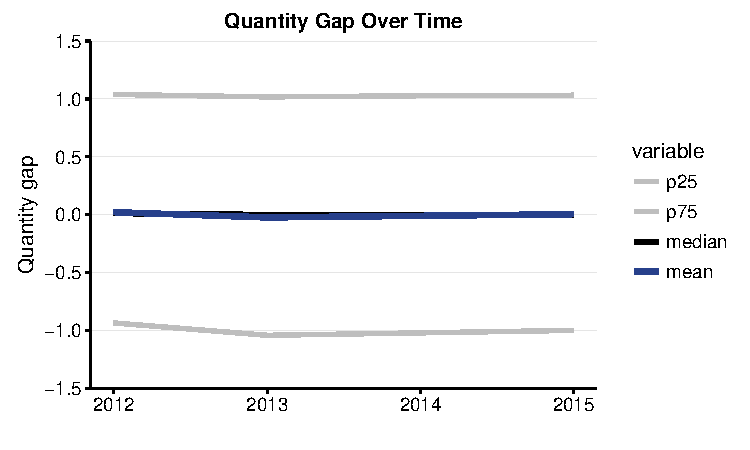
\includegraphics{Figs/qty_summary-1} \end{center}

\begin{Shaded}
\begin{Highlighting}[]
\CommentTok{#Across products?}
\NormalTok{products <-}\StringTok{ }\NormalTok{hs12_all_tariffs[, .(}\DataTypeTok{mean =} \KeywordTok{as.double}\NormalTok{(}\KeywordTok{mean}\NormalTok{(Qty_log_gap)),}
                                 \DataTypeTok{median =} \KeywordTok{as.double}\NormalTok{(}\KeywordTok{median}\NormalTok{(Qty_log_gap)),}
                                 \DataTypeTok{p25 =} \KeywordTok{as.double}\NormalTok{(}\KeywordTok{quantile}\NormalTok{(Qty_log_gap,.}\DecValTok{25}\NormalTok{)),}
                                 \DataTypeTok{p75 =} \KeywordTok{as.double}\NormalTok{(}\KeywordTok{quantile}\NormalTok{(Qty_log_gap,.}\DecValTok{75}\NormalTok{))}
\NormalTok{),}
\NormalTok{by=}\StringTok{ }\NormalTok{ProductCode]}

\KeywordTok{ggplot}\NormalTok{(}\DataTypeTok{data=}\NormalTok{products, }\KeywordTok{aes}\NormalTok{(mean)) +}
\StringTok{  }\KeywordTok{geom_histogram}\NormalTok{(}\DataTypeTok{col=}\StringTok{"royalblue4"}\NormalTok{,}
                 \DataTypeTok{fill=}\StringTok{"royalblue4"}\NormalTok{,}
                 \DataTypeTok{alpha=}\NormalTok{.}\DecValTok{2}\NormalTok{) +}
\StringTok{  }\KeywordTok{background_grid}\NormalTok{(}\DataTypeTok{major =} \StringTok{'y'}\NormalTok{, }\DataTypeTok{minor =} \StringTok{"none"}\NormalTok{) +}
\StringTok{  }\KeywordTok{scale_y_continuous}\NormalTok{(}\DataTypeTok{expand =} \KeywordTok{c}\NormalTok{(}\DecValTok{0}\NormalTok{, }\DecValTok{0}\NormalTok{), }\DataTypeTok{limits =} \KeywordTok{c}\NormalTok{(}\DecValTok{0}\NormalTok{, }\DecValTok{3000}\NormalTok{))  +}
\StringTok{  }\KeywordTok{labs}\NormalTok{(}\DataTypeTok{title=}\StringTok{"Mean Quantity Gap Across Products"}\NormalTok{) +}
\StringTok{  }\KeywordTok{labs}\NormalTok{(}\DataTypeTok{x=}\StringTok{"Quantity gap"}\NormalTok{, }\DataTypeTok{y=}\StringTok{"Number of products"}\NormalTok{)}
\end{Highlighting}
\end{Shaded}

\begin{center}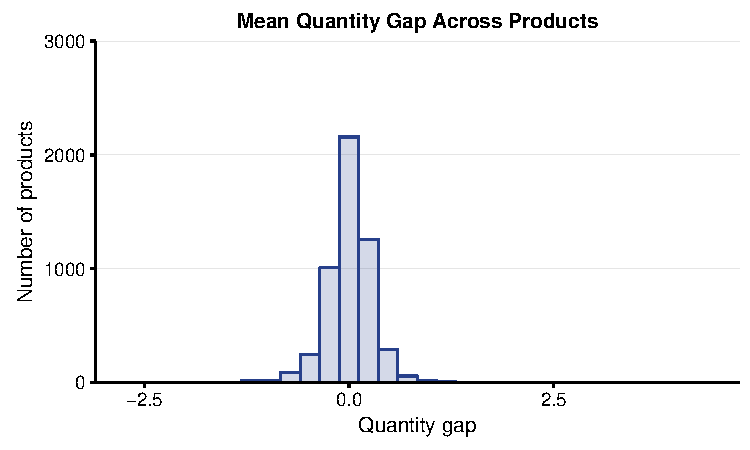
\includegraphics{Figs/qty_summary-2} \end{center}

\begin{Shaded}
\begin{Highlighting}[]
\KeywordTok{ggplot}\NormalTok{(}\DataTypeTok{data=}\NormalTok{products, }\KeywordTok{aes}\NormalTok{(median)) +}
\StringTok{  }\KeywordTok{geom_histogram}\NormalTok{(}\DataTypeTok{col=}\StringTok{"royalblue4"}\NormalTok{,}
                 \DataTypeTok{fill=}\StringTok{"royalblue4"}\NormalTok{,}
                 \DataTypeTok{alpha=}\NormalTok{.}\DecValTok{2}\NormalTok{) +}
\StringTok{  }\KeywordTok{background_grid}\NormalTok{(}\DataTypeTok{major =} \StringTok{'y'}\NormalTok{, }\DataTypeTok{minor =} \StringTok{"none"}\NormalTok{) +}
\StringTok{  }\KeywordTok{scale_y_continuous}\NormalTok{(}\DataTypeTok{expand =} \KeywordTok{c}\NormalTok{(}\DecValTok{0}\NormalTok{, }\DecValTok{0}\NormalTok{), }\DataTypeTok{limits =} \KeywordTok{c}\NormalTok{(}\DecValTok{0}\NormalTok{, }\DecValTok{5000}\NormalTok{)) +}
\StringTok{  }\KeywordTok{labs}\NormalTok{(}\DataTypeTok{title=}\StringTok{"Median Quantity Gap Across Products"}\NormalTok{) +}
\StringTok{  }\KeywordTok{labs}\NormalTok{(}\DataTypeTok{x=}\StringTok{"Quantity gap"}\NormalTok{, }\DataTypeTok{y=}\StringTok{"Number of products"}\NormalTok{)}
\end{Highlighting}
\end{Shaded}

\begin{center}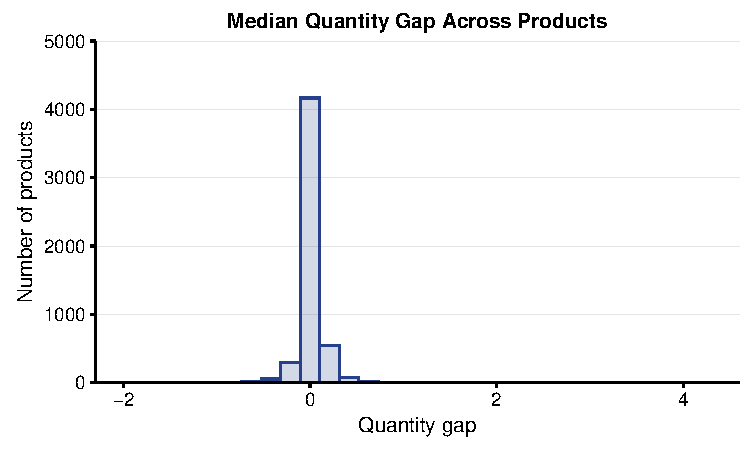
\includegraphics{Figs/qty_summary-3} \end{center}

\begin{Shaded}
\begin{Highlighting}[]
\KeywordTok{ggplot}\NormalTok{(}\DataTypeTok{data=}\NormalTok{products, }\KeywordTok{aes}\NormalTok{(p25)) +}
\StringTok{  }\KeywordTok{geom_histogram}\NormalTok{(}\DataTypeTok{col=}\StringTok{"royalblue4"}\NormalTok{,}
                 \DataTypeTok{fill=}\StringTok{"royalblue4"}\NormalTok{,}
                 \DataTypeTok{alpha=}\NormalTok{.}\DecValTok{2}\NormalTok{) +}
\StringTok{  }\KeywordTok{background_grid}\NormalTok{(}\DataTypeTok{major =} \StringTok{'y'}\NormalTok{, }\DataTypeTok{minor =} \StringTok{"none"}\NormalTok{) +}
\StringTok{  }\KeywordTok{scale_y_continuous}\NormalTok{(}\DataTypeTok{expand =} \KeywordTok{c}\NormalTok{(}\DecValTok{0}\NormalTok{, }\DecValTok{0}\NormalTok{), }\DataTypeTok{limits =} \KeywordTok{c}\NormalTok{(}\DecValTok{0}\NormalTok{,}\DecValTok{2000}\NormalTok{),  }\DataTypeTok{minor_breaks =} \OtherTok{NULL}\NormalTok{) +}
\StringTok{  }\KeywordTok{labs}\NormalTok{(}\DataTypeTok{title=}\StringTok{"25th Percentile Quantity Gap Across Products"}\NormalTok{) +}
\StringTok{  }\KeywordTok{labs}\NormalTok{(}\DataTypeTok{x=}\StringTok{"Quantity gap"}\NormalTok{, }\DataTypeTok{y=}\StringTok{"Number of products"}\NormalTok{)}
\end{Highlighting}
\end{Shaded}

\begin{center}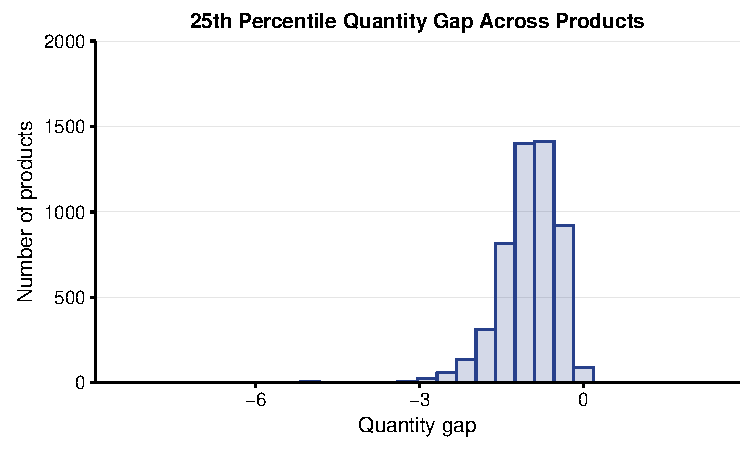
\includegraphics{Figs/qty_summary-4} \end{center}

\begin{Shaded}
\begin{Highlighting}[]
\KeywordTok{ggplot}\NormalTok{(}\DataTypeTok{data=}\NormalTok{products, }\KeywordTok{aes}\NormalTok{(p75)) +}
\StringTok{  }\KeywordTok{geom_histogram}\NormalTok{(}\DataTypeTok{col=}\StringTok{"royalblue4"}\NormalTok{,}
                 \DataTypeTok{fill=}\StringTok{"royalblue4"}\NormalTok{,}
                 \DataTypeTok{alpha=}\NormalTok{.}\DecValTok{2}\NormalTok{) +}
\StringTok{  }\KeywordTok{background_grid}\NormalTok{(}\DataTypeTok{major =} \StringTok{'y'}\NormalTok{, }\DataTypeTok{minor =} \StringTok{"none"}\NormalTok{) +}
\StringTok{  }\KeywordTok{scale_y_continuous}\NormalTok{(}\DataTypeTok{expand =} \KeywordTok{c}\NormalTok{(}\DecValTok{0}\NormalTok{, }\DecValTok{0}\NormalTok{),  }\DataTypeTok{limits =} \KeywordTok{c}\NormalTok{(}\DecValTok{0}\NormalTok{, }\DecValTok{2000}\NormalTok{), }\DataTypeTok{minor_breaks =} \OtherTok{NULL}\NormalTok{) +}
\StringTok{  }\KeywordTok{labs}\NormalTok{(}\DataTypeTok{title=}\StringTok{"75th Percentile Quantity Gap Across Products"}\NormalTok{) +}
\StringTok{  }\KeywordTok{labs}\NormalTok{(}\DataTypeTok{x=}\StringTok{"Quantity gap"}\NormalTok{, }\DataTypeTok{y=}\StringTok{"Number of products"}\NormalTok{)}
\end{Highlighting}
\end{Shaded}

\begin{center}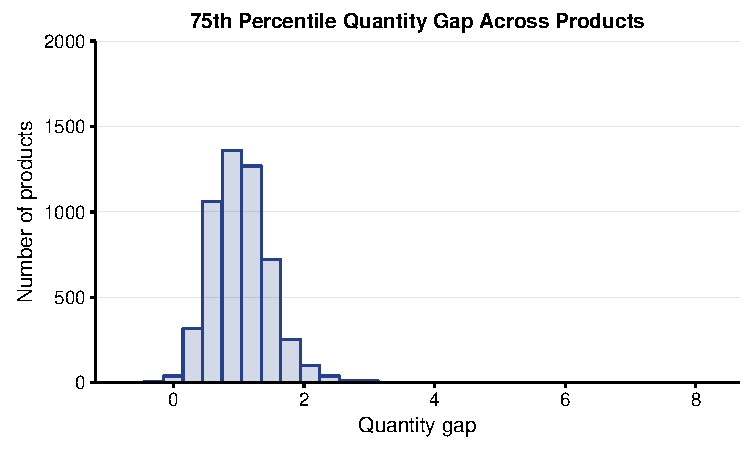
\includegraphics{Figs/qty_summary-5} \end{center}

\begin{Shaded}
\begin{Highlighting}[]
\CommentTok{#Across countries?}
\NormalTok{countries <-}\StringTok{ }\NormalTok{hs12_all_tariffs[, .(}\DataTypeTok{mean =} \KeywordTok{as.double}\NormalTok{(}\KeywordTok{mean}\NormalTok{(Qty_log_gap)),}
                                  \DataTypeTok{median =} \KeywordTok{as.double}\NormalTok{(}\KeywordTok{median}\NormalTok{(Qty_log_gap)),}
                                  \DataTypeTok{p25 =} \KeywordTok{as.double}\NormalTok{(}\KeywordTok{quantile}\NormalTok{(Qty_log_gap,.}\DecValTok{25}\NormalTok{)),}
                                  \DataTypeTok{p75 =} \KeywordTok{as.double}\NormalTok{(}\KeywordTok{quantile}\NormalTok{(Qty_log_gap,.}\DecValTok{75}\NormalTok{))}
\NormalTok{),}
\NormalTok{by=}\StringTok{ }\KeywordTok{c}\NormalTok{(}\StringTok{"Importer"}\NormalTok{, }\StringTok{"Exporter"}\NormalTok{)]}

\KeywordTok{ggplot}\NormalTok{(}\DataTypeTok{data=}\NormalTok{countries, }\KeywordTok{aes}\NormalTok{(mean)) +}
\StringTok{  }\KeywordTok{geom_histogram}\NormalTok{(}\DataTypeTok{col=}\StringTok{"royalblue4"}\NormalTok{,}
                 \DataTypeTok{fill=}\StringTok{"royalblue4"}\NormalTok{,}
                 \DataTypeTok{alpha=}\NormalTok{.}\DecValTok{2}\NormalTok{) +}
\StringTok{  }\KeywordTok{background_grid}\NormalTok{(}\DataTypeTok{major =} \StringTok{'y'}\NormalTok{, }\DataTypeTok{minor =} \StringTok{"none"}\NormalTok{) +}
\StringTok{  }\KeywordTok{scale_y_continuous}\NormalTok{(}\DataTypeTok{expand =} \KeywordTok{c}\NormalTok{(}\DecValTok{0}\NormalTok{, }\DecValTok{0}\NormalTok{), }\DataTypeTok{limits =} \KeywordTok{c}\NormalTok{(}\DecValTok{0}\NormalTok{, }\DecValTok{5000}\NormalTok{),  }\DataTypeTok{minor_breaks =} \OtherTok{NULL}\NormalTok{) +}
\StringTok{  }\KeywordTok{labs}\NormalTok{(}\DataTypeTok{title=}\StringTok{"Mean Quantity Gap Across Country Pairs"}\NormalTok{) +}
\StringTok{  }\KeywordTok{labs}\NormalTok{(}\DataTypeTok{x=}\StringTok{"Quantity gap"}\NormalTok{, }\DataTypeTok{y=}\StringTok{"Number of pairs"}\NormalTok{)}
\end{Highlighting}
\end{Shaded}

\begin{center}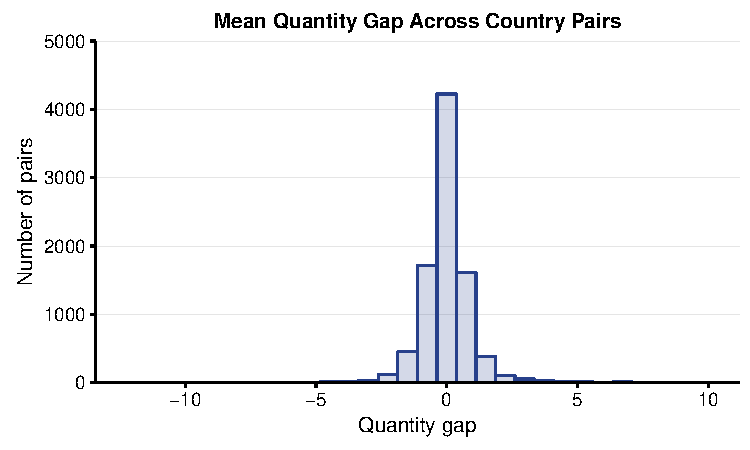
\includegraphics{Figs/qty_summary-6} \end{center}

\begin{Shaded}
\begin{Highlighting}[]
\KeywordTok{ggplot}\NormalTok{(}\DataTypeTok{data=}\NormalTok{countries, }\KeywordTok{aes}\NormalTok{(median)) +}
\StringTok{  }\KeywordTok{geom_histogram}\NormalTok{(}\DataTypeTok{col=}\StringTok{"royalblue4"}\NormalTok{,}
                 \DataTypeTok{fill=}\StringTok{"royalblue4"}\NormalTok{,}
                 \DataTypeTok{alpha=}\NormalTok{.}\DecValTok{2}\NormalTok{) +}
\StringTok{  }\KeywordTok{background_grid}\NormalTok{(}\DataTypeTok{major =} \StringTok{'y'}\NormalTok{, }\DataTypeTok{minor =} \StringTok{"none"}\NormalTok{) +}
\StringTok{  }\KeywordTok{scale_y_continuous}\NormalTok{(}\DataTypeTok{expand =} \KeywordTok{c}\NormalTok{(}\DecValTok{0}\NormalTok{, }\DecValTok{0}\NormalTok{), }\DataTypeTok{limits =} \KeywordTok{c}\NormalTok{(}\DecValTok{0}\NormalTok{, }\DecValTok{6000}\NormalTok{), }\DataTypeTok{minor_breaks =} \OtherTok{NULL}\NormalTok{) +}
\StringTok{  }\KeywordTok{labs}\NormalTok{(}\DataTypeTok{title=}\StringTok{"Median Quantity Gap Across Country Pairs"}\NormalTok{) +}
\StringTok{  }\KeywordTok{labs}\NormalTok{(}\DataTypeTok{x=}\StringTok{"Quantity gap"}\NormalTok{, }\DataTypeTok{y=}\StringTok{"Number of pairs"}\NormalTok{)}
\end{Highlighting}
\end{Shaded}

\begin{center}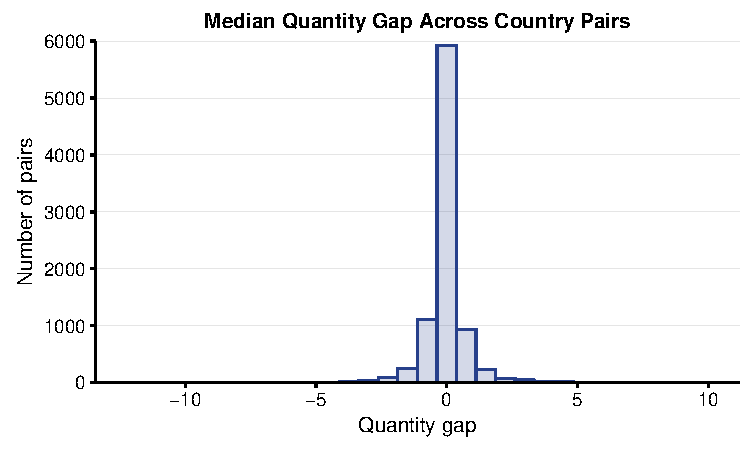
\includegraphics{Figs/qty_summary-7} \end{center}

\begin{Shaded}
\begin{Highlighting}[]
\KeywordTok{ggplot}\NormalTok{(}\DataTypeTok{data=}\NormalTok{countries, }\KeywordTok{aes}\NormalTok{(p25)) +}
\StringTok{  }\KeywordTok{geom_histogram}\NormalTok{(}\DataTypeTok{col=}\StringTok{"royalblue4"}\NormalTok{,}
                 \DataTypeTok{fill=}\StringTok{"royalblue4"}\NormalTok{,}
                 \DataTypeTok{alpha=}\NormalTok{.}\DecValTok{2}\NormalTok{) +}
\StringTok{  }\KeywordTok{background_grid}\NormalTok{(}\DataTypeTok{major =} \StringTok{'y'}\NormalTok{, }\DataTypeTok{minor =} \StringTok{"none"}\NormalTok{) +}
\StringTok{  }\KeywordTok{scale_y_continuous}\NormalTok{(}\DataTypeTok{expand =} \KeywordTok{c}\NormalTok{(}\DecValTok{0}\NormalTok{, }\DecValTok{0}\NormalTok{), }\DataTypeTok{limits =} \KeywordTok{c}\NormalTok{(}\DecValTok{0}\NormalTok{, }\DecValTok{4000}\NormalTok{),  }\DataTypeTok{minor_breaks =} \OtherTok{NULL}\NormalTok{) +}
\StringTok{  }\KeywordTok{labs}\NormalTok{(}\DataTypeTok{title=}\StringTok{"25th Percentile Quantity Gap Across Country Pairs"}\NormalTok{) +}
\StringTok{  }\KeywordTok{labs}\NormalTok{(}\DataTypeTok{x=}\StringTok{"Quantity gap"}\NormalTok{, }\DataTypeTok{y=}\StringTok{"Number of pairs"}\NormalTok{)}
\end{Highlighting}
\end{Shaded}

\begin{center}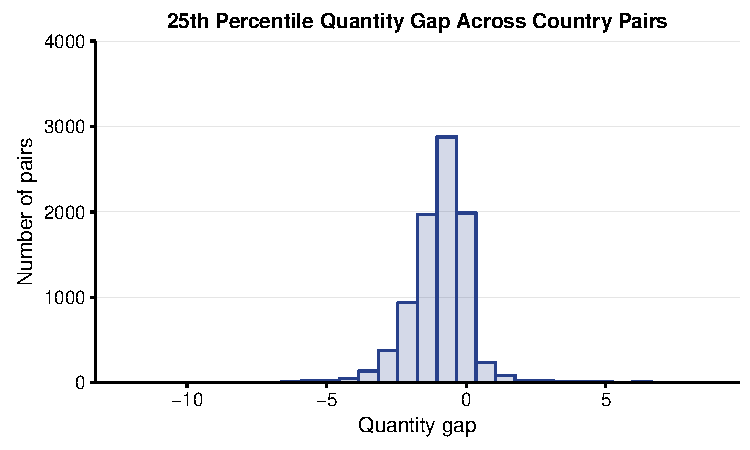
\includegraphics{Figs/qty_summary-8} \end{center}

\begin{Shaded}
\begin{Highlighting}[]
\KeywordTok{ggplot}\NormalTok{(}\DataTypeTok{data=}\NormalTok{countries, }\KeywordTok{aes}\NormalTok{(p75)) +}
\StringTok{  }\KeywordTok{geom_histogram}\NormalTok{(}\DataTypeTok{col=}\StringTok{"royalblue4"}\NormalTok{,}
                 \DataTypeTok{fill=}\StringTok{"royalblue4"}\NormalTok{,}
                 \DataTypeTok{alpha=}\NormalTok{.}\DecValTok{2}\NormalTok{) +}
\StringTok{  }\KeywordTok{background_grid}\NormalTok{(}\DataTypeTok{major =} \StringTok{'y'}\NormalTok{, }\DataTypeTok{minor =} \StringTok{"none"}\NormalTok{) +}
\StringTok{  }\KeywordTok{scale_y_continuous}\NormalTok{(}\DataTypeTok{expand =} \KeywordTok{c}\NormalTok{(}\DecValTok{0}\NormalTok{, }\DecValTok{0}\NormalTok{), }\DataTypeTok{limits =} \KeywordTok{c}\NormalTok{(}\DecValTok{0}\NormalTok{, }\DecValTok{4000}\NormalTok{),  }\DataTypeTok{minor_breaks =} \OtherTok{NULL}\NormalTok{) +}
\StringTok{  }\KeywordTok{labs}\NormalTok{(}\DataTypeTok{title=}\StringTok{"75th Percentile Quantity Gap Across Country Pairs"}\NormalTok{) +}
\StringTok{  }\KeywordTok{labs}\NormalTok{(}\DataTypeTok{x=}\StringTok{"Quantity gap"}\NormalTok{, }\DataTypeTok{y=}\StringTok{"Number of pairs"}\NormalTok{)}
\end{Highlighting}
\end{Shaded}

\begin{center}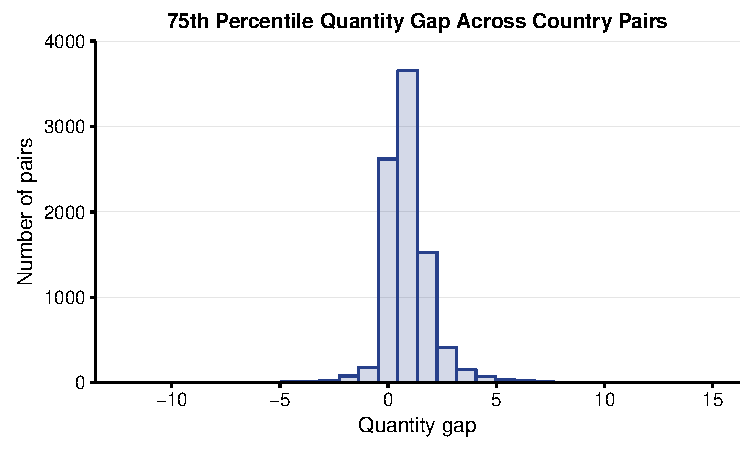
\includegraphics{Figs/qty_summary-9} \end{center}

\begin{Shaded}
\begin{Highlighting}[]
\KeywordTok{rm}\NormalTok{(Years, products, countries, hs12_all_tariffs)}

\CommentTok{#Regress trade gap on dummies and plot coefficients }

\KeywordTok{load}\NormalTok{(}\KeywordTok{paste}\NormalTok{(DataPath,}\StringTok{"Analysis Data/hs12_all_tariffs_qty.Rda"}\NormalTok{, }\DataTypeTok{sep =} \StringTok{"/"}\NormalTok{))}

\NormalTok{hs12_all_tariffs <-}\StringTok{ }\NormalTok{hs12_all_tariffs[, .(Year, ProductCode, }\StringTok{`}\DataTypeTok{Reporter_ISO_N}\StringTok{`}\NormalTok{, }\StringTok{`}\DataTypeTok{Partner Code}\StringTok{`}\NormalTok{, Qty_log_gap)]}

\NormalTok{hs12_all_tariffs$Year <-}\StringTok{ }\KeywordTok{as.Date}\NormalTok{(hs12_all_tariffs$Year, }\StringTok{"%Y"}\NormalTok{)}
\NormalTok{hs12_all_tariffs$Year <-}\StringTok{ }\KeywordTok{floor_date}\NormalTok{(hs12_all_tariffs$Year,}\StringTok{"year"}\NormalTok{)}

\NormalTok{hs12_all_tariffs$Year.f <-}\StringTok{ }\KeywordTok{factor}\NormalTok{(hs12_all_tariffs$Year)}
\NormalTok{hs12_all_tariffs$Products.f <-}\StringTok{ }\KeywordTok{factor}\NormalTok{(hs12_all_tariffs$ProductCode)}

\NormalTok{hs12_all_tariffs$Importer.f <-}\StringTok{ }\KeywordTok{factor}\NormalTok{(hs12_all_tariffs$}\StringTok{`}\DataTypeTok{Reporter_ISO_N}\StringTok{`}\NormalTok{)}
\NormalTok{hs12_all_tariffs$Exporter.f <-}\StringTok{ }\KeywordTok{factor}\NormalTok{(hs12_all_tariffs$}\StringTok{`}\DataTypeTok{Partner Code}\StringTok{`}\NormalTok{)}
\NormalTok{hs12_all_tariffs$Pairs.f <-}\StringTok{ }\KeywordTok{with}\NormalTok{(hs12_all_tariffs, }\KeywordTok{interaction}\NormalTok{(Importer.f, Exporter.f))}

\NormalTok{hs12_all_tariffs <-}\StringTok{ }\NormalTok{hs12_all_tariffs[, .(Year, Qty_log_gap, Year.f, Products.f, Pairs.f)]}

\NormalTok{reg <-}\StringTok{ }\KeywordTok{felm}\NormalTok{(Qty_log_gap ~}\StringTok{ }\DecValTok{1} \NormalTok{|}\StringTok{ }\NormalTok{Year.f +}\StringTok{ }\NormalTok{Products.f +}\StringTok{ }\NormalTok{Pairs.f,}
            \DataTypeTok{data =} \NormalTok{hs12_all_tariffs,}
            \DataTypeTok{exactDOF =} \OtherTok{FALSE}\NormalTok{,}
            \DataTypeTok{keepX =} \OtherTok{FALSE}\NormalTok{,}
            \DataTypeTok{keepCX =} \OtherTok{FALSE}\NormalTok{)}

\NormalTok{fes <-}\StringTok{ }\KeywordTok{getfe}\NormalTok{(reg,}
             \DataTypeTok{se=}\OtherTok{TRUE}\NormalTok{,}
             \DataTypeTok{bN =} \DecValTok{50}
\NormalTok{)}

\NormalTok{Yearfes <-}\StringTok{ }\KeywordTok{subset}\NormalTok{(fes,fe ==}\StringTok{ "Year.f"}\NormalTok{)}

\NormalTok{Yearfes$ci_ub <-}\StringTok{ }\NormalTok{Yearfes$effect +}\StringTok{ }\NormalTok{(}\FloatTok{1.96} \NormalTok{*}\StringTok{ }\NormalTok{Yearfes$se)}
\NormalTok{Yearfes$ci_lb <-}\StringTok{ }\NormalTok{Yearfes$effect -}\StringTok{ }\NormalTok{(}\FloatTok{1.96} \NormalTok{*}\StringTok{ }\NormalTok{Yearfes$se)}
\NormalTok{Yearfes <-}\StringTok{ }\KeywordTok{merge}\NormalTok{(Yearfes,}\KeywordTok{unique}\NormalTok{(hs12_all_tariffs[,}\KeywordTok{list}\NormalTok{(Year,Year.f)]),}\DataTypeTok{by.x =} \StringTok{"idx"}\NormalTok{,}\DataTypeTok{by.y=}\StringTok{"Year.f"}\NormalTok{)}
\NormalTok{Yearfes <-}\StringTok{ }\KeywordTok{rename}\NormalTok{(Yearfes, }\DataTypeTok{Year =} \NormalTok{Year)}

\KeywordTok{ggplot}\NormalTok{(}\DataTypeTok{data =} \NormalTok{Yearfes, }\KeywordTok{aes}\NormalTok{(Year,effect)) +}
\StringTok{  }\KeywordTok{geom_errorbar}\NormalTok{(}\KeywordTok{aes}\NormalTok{(}\DataTypeTok{ymin =} \NormalTok{ci_lb, }\DataTypeTok{ymax =} \NormalTok{ci_ub), }\DataTypeTok{color =} \StringTok{"grey35"}\NormalTok{) +}
\StringTok{  }\KeywordTok{geom_line}\NormalTok{(}\DataTypeTok{color =} \StringTok{"royalblue4"}\NormalTok{, }\DataTypeTok{size =} \DecValTok{1}\NormalTok{) +}
\StringTok{  }\KeywordTok{geom_point}\NormalTok{(}\DataTypeTok{color =} \StringTok{"royalblue4"}\NormalTok{) +}
\StringTok{  }\KeywordTok{background_grid}\NormalTok{(}\DataTypeTok{major =} \StringTok{'y'}\NormalTok{, }\DataTypeTok{minor =} \StringTok{"none"}\NormalTok{) +}
\StringTok{  }\KeywordTok{scale_y_continuous}\NormalTok{(}\DataTypeTok{expand =} \KeywordTok{c}\NormalTok{(}\DecValTok{0}\NormalTok{, }\DecValTok{0}\NormalTok{), }\DataTypeTok{limits =} \KeywordTok{c}\NormalTok{(-.}\DecValTok{05}\NormalTok{,.}\DecValTok{05}\NormalTok{), }\DataTypeTok{minor_breaks =} \OtherTok{NULL}\NormalTok{) +}
\StringTok{  }\KeywordTok{xlab}\NormalTok{(}\DataTypeTok{label =} \StringTok{""}\NormalTok{) +}
\StringTok{  }\KeywordTok{ylab}\NormalTok{(}\DataTypeTok{label =} \StringTok{"Quantity gap"}\NormalTok{) +}
\StringTok{  }\KeywordTok{labs}\NormalTok{(}\DataTypeTok{title =} \StringTok{"Quantity Gap Over Time, Controlling for Product/Country Pairs"}\NormalTok{)}
\end{Highlighting}
\end{Shaded}

\begin{center}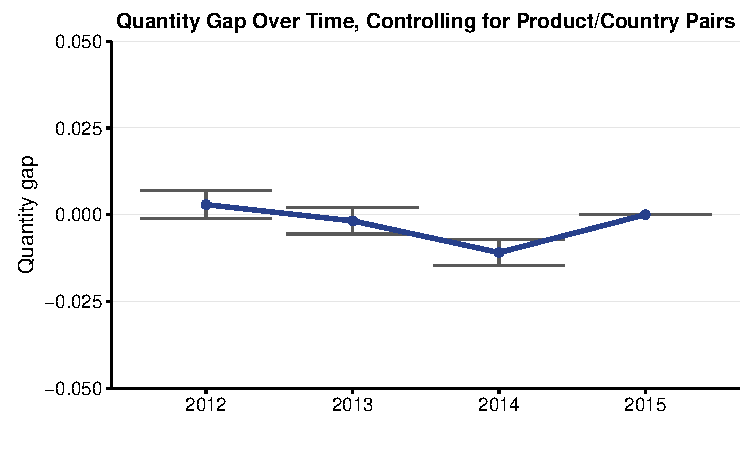
\includegraphics{Figs/qty_summary-10} \end{center}

\begin{Shaded}
\begin{Highlighting}[]
\NormalTok{productfes <-}\StringTok{ }\KeywordTok{subset}\NormalTok{(fes,fe ==}\StringTok{ "Products.f"}\NormalTok{)}
\NormalTok{productfes <-}\StringTok{ }\NormalTok{productfes[,}\KeywordTok{c}\NormalTok{(}\StringTok{"effect"}\NormalTok{,}\StringTok{"idx"}\NormalTok{)]}

\KeywordTok{ggplot}\NormalTok{(}\DataTypeTok{data=}\NormalTok{productfes, }\KeywordTok{aes}\NormalTok{(effect)) +}
\StringTok{  }\KeywordTok{geom_histogram}\NormalTok{(}\DataTypeTok{col=}\StringTok{"royalblue4"}\NormalTok{,}
                 \DataTypeTok{fill=}\StringTok{"royalblue4"}\NormalTok{,}
                 \DataTypeTok{alpha=}\NormalTok{.}\DecValTok{2}\NormalTok{) +}
\StringTok{  }\KeywordTok{background_grid}\NormalTok{(}\DataTypeTok{major =} \StringTok{'y'}\NormalTok{, }\DataTypeTok{minor =} \StringTok{"none"}\NormalTok{) +}
\StringTok{  }\KeywordTok{scale_y_continuous}\NormalTok{(}\DataTypeTok{expand =} \KeywordTok{c}\NormalTok{(}\DecValTok{0}\NormalTok{, }\DecValTok{0}\NormalTok{), }\DataTypeTok{limits =} \KeywordTok{c}\NormalTok{(}\DecValTok{0}\NormalTok{,}\DecValTok{2000}\NormalTok{), }\DataTypeTok{minor_breaks =} \OtherTok{NULL}\NormalTok{) +}
\StringTok{  }\KeywordTok{labs}\NormalTok{(}\DataTypeTok{title=}\StringTok{"Mean Quantity Gap Across Products, Controlling for Country Pairs/Years"}\NormalTok{) +}
\StringTok{  }\KeywordTok{labs}\NormalTok{(}\DataTypeTok{x=}\StringTok{"Quantity gap"}\NormalTok{, }\DataTypeTok{y=}\StringTok{"Number of products"}\NormalTok{)}
\end{Highlighting}
\end{Shaded}

\begin{center}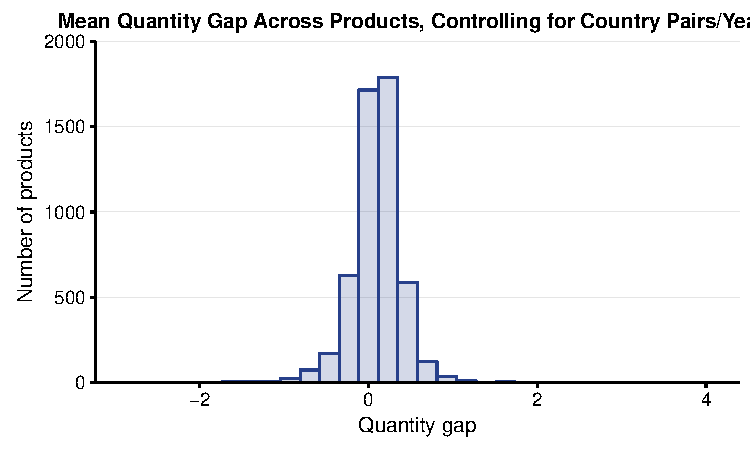
\includegraphics{Figs/qty_summary-11} \end{center}

\begin{Shaded}
\begin{Highlighting}[]
\NormalTok{pairfes <-}\StringTok{ }\KeywordTok{subset}\NormalTok{(fes,fe ==}\StringTok{ "Pairs.f"}\NormalTok{)}
\NormalTok{pairfes <-}\StringTok{ }\NormalTok{pairfes[,}\KeywordTok{c}\NormalTok{(}\StringTok{"effect"}\NormalTok{,}\StringTok{"idx"}\NormalTok{)]}

\KeywordTok{ggplot}\NormalTok{(}\DataTypeTok{data=}\NormalTok{pairfes, }\KeywordTok{aes}\NormalTok{(effect)) +}
\StringTok{  }\KeywordTok{geom_histogram}\NormalTok{(}\DataTypeTok{col=}\StringTok{"royalblue4"}\NormalTok{,}
                 \DataTypeTok{fill=}\StringTok{"royalblue4"}\NormalTok{,}
                 \DataTypeTok{alpha=}\NormalTok{.}\DecValTok{2}\NormalTok{) +}
\StringTok{  }\KeywordTok{background_grid}\NormalTok{(}\DataTypeTok{major =} \StringTok{'y'}\NormalTok{, }\DataTypeTok{minor =} \StringTok{"none"}\NormalTok{) +}
\StringTok{  }\KeywordTok{scale_y_continuous}\NormalTok{(}\DataTypeTok{expand =} \KeywordTok{c}\NormalTok{(}\DecValTok{0}\NormalTok{, }\DecValTok{0}\NormalTok{), }\DataTypeTok{limits =} \KeywordTok{c}\NormalTok{(}\DecValTok{0}\NormalTok{, }\DecValTok{5000}\NormalTok{), }\DataTypeTok{minor_breaks =} \OtherTok{NULL}\NormalTok{) +}
\StringTok{  }\KeywordTok{labs}\NormalTok{(}\DataTypeTok{title=}\StringTok{"Mean Quantity Gap Across Country Pairs, Controlling for Products/Years"}\NormalTok{) +}
\StringTok{  }\KeywordTok{labs}\NormalTok{(}\DataTypeTok{x=}\StringTok{"Quantity gap"}\NormalTok{, }\DataTypeTok{y=}\StringTok{"Number of country pairs"}\NormalTok{)}
\end{Highlighting}
\end{Shaded}

\begin{center}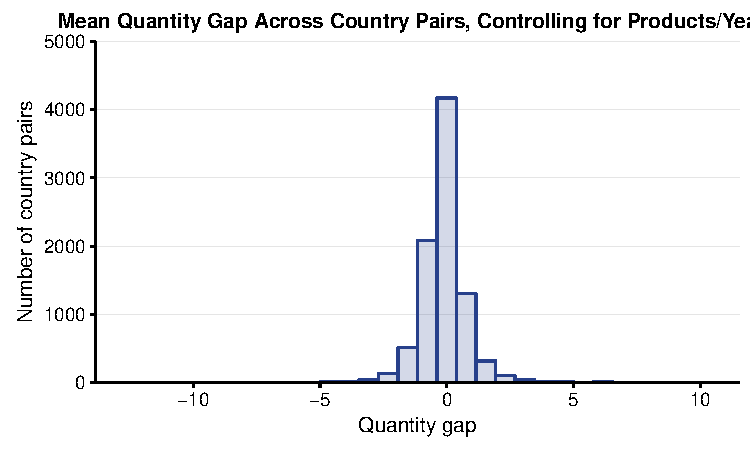
\includegraphics{Figs/qty_summary-12} \end{center}

\begin{Shaded}
\begin{Highlighting}[]
\KeywordTok{rm}\NormalTok{(fes, hs12_all_tariffs, pairfes, Yearfes, productfes, reg)}
\end{Highlighting}
\end{Shaded}

\section{Tariff Data Summary}\label{tariff-data-summary}

The following figure presents preferential tariffs as a share of each
country's total tariffs, for data that matches with the quantity trade
data.

\begin{Shaded}
\begin{Highlighting}[]
\KeywordTok{load}\NormalTok{(}\KeywordTok{paste}\NormalTok{(DataPath,}\StringTok{"Analysis Data/hs12_all_tariffs_qty.Rda"}\NormalTok{, }\DataTypeTok{sep =} \StringTok{"/"}\NormalTok{))}

\NormalTok{hs12_all_tariffs <-}\StringTok{ }\NormalTok{hs12_all_tariffs[, .(Year, ProductCode, Importer, Exporter, pref)]}

\NormalTok{pref <-}\StringTok{ }\NormalTok{hs12_all_tariffs[pref==}\DecValTok{1}\NormalTok{, .N, by =}\StringTok{ }\KeywordTok{c}\NormalTok{(}\StringTok{"Importer"}\NormalTok{)]}
\NormalTok{pref <-}\StringTok{ }\KeywordTok{rename}\NormalTok{(pref, }\StringTok{"Pref"} \NormalTok{=}\StringTok{ "N"}\NormalTok{)}

\NormalTok{mfn <-}\StringTok{ }\NormalTok{hs12_all_tariffs[}\KeywordTok{is.na}\NormalTok{(pref), .N, by =}\StringTok{ }\KeywordTok{c}\NormalTok{(}\StringTok{"Importer"}\NormalTok{)]}
\NormalTok{mfn <-}\StringTok{ }\KeywordTok{rename}\NormalTok{(mfn, }\StringTok{"MFN"} \NormalTok{=}\StringTok{ "N"}\NormalTok{)}

\NormalTok{tariffs <-}\StringTok{ }\KeywordTok{merge}\NormalTok{(pref, mfn, }\DataTypeTok{by =} \KeywordTok{c}\NormalTok{(}\StringTok{"Importer"}\NormalTok{), }\DataTypeTok{all =} \NormalTok{T)}

\NormalTok{tariffs[}\KeywordTok{is.na}\NormalTok{(tariffs)] <-}\StringTok{ }\DecValTok{0}

\NormalTok{tariffs$All <-}\StringTok{ }\NormalTok{tariffs$Pref +}\StringTok{ }\NormalTok{tariffs$MFN}
\NormalTok{tariffs$Share_pref <-}\StringTok{ }\NormalTok{tariffs$Pref /}\StringTok{ }\NormalTok{tariffs$All}

\KeywordTok{ggplot}\NormalTok{(tariffs, }\KeywordTok{aes}\NormalTok{(Share_pref)) +}
\StringTok{  }\KeywordTok{geom_histogram}\NormalTok{(}\DataTypeTok{col=}\StringTok{"royalblue4"}\NormalTok{,}
                 \DataTypeTok{fill=}\StringTok{"royalblue4"}\NormalTok{,}
                 \DataTypeTok{bins =} \DecValTok{10}\NormalTok{,}
                 \DataTypeTok{alpha=}\NormalTok{.}\DecValTok{2}\NormalTok{) +}
\StringTok{  }\KeywordTok{background_grid}\NormalTok{(}\DataTypeTok{major =} \StringTok{'y'}\NormalTok{, }\DataTypeTok{minor =} \StringTok{"none"}\NormalTok{) +}
\StringTok{  }\KeywordTok{scale_y_continuous}\NormalTok{(}\DataTypeTok{expand =} \KeywordTok{c}\NormalTok{(}\DecValTok{0}\NormalTok{, }\DecValTok{0}\NormalTok{), }\DataTypeTok{limits =} \KeywordTok{c}\NormalTok{(}\DecValTok{0}\NormalTok{, }\DecValTok{25}\NormalTok{), }\DataTypeTok{minor_breaks =} \OtherTok{NULL}\NormalTok{) +}
\StringTok{  }\KeywordTok{labs}\NormalTok{(}\DataTypeTok{title=}\StringTok{"Preferential Tariffs as a Share of Total"}\NormalTok{) +}
\StringTok{  }\KeywordTok{labs}\NormalTok{(}\DataTypeTok{x=}\StringTok{"Share of all tariffs"}\NormalTok{, }\DataTypeTok{y=}\StringTok{"Number of importers"}\NormalTok{)}
\end{Highlighting}
\end{Shaded}

\begin{center}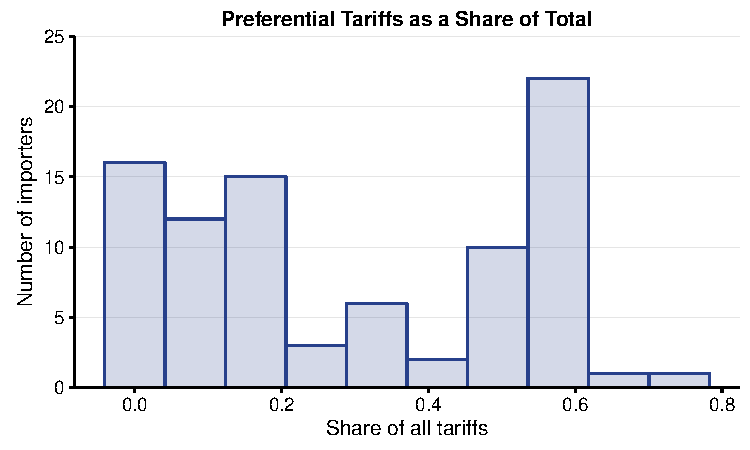
\includegraphics{Figs/pref_summary-1} \end{center}

\begin{Shaded}
\begin{Highlighting}[]
\KeywordTok{rm}\NormalTok{(hs12_all_tariffs, mfn, pref, tariffs)}
\end{Highlighting}
\end{Shaded}

The next section summarizes the ``Simple Average'' tariff rate as
reported by WITS, for tariffs that match with the quantity trade data.
The Simple Average is the average ad valorem tariff rate within each
six-digit HS code. Each tariff is the most-favored nation rate unless
there is a corresponding preferential tariff rate. There were some
instances of multiple preferential tariff rates, in which case I took
the lowest value if the average was different.

\begin{Shaded}
\begin{Highlighting}[]
\KeywordTok{load}\NormalTok{(}\KeywordTok{paste}\NormalTok{(DataPath,}\StringTok{"Analysis Data/hs12_all_tariffs_qty.Rda"}\NormalTok{, }\DataTypeTok{sep =} \StringTok{"/"}\NormalTok{))}

\NormalTok{hs12_all_tariffs <-}\StringTok{ }\NormalTok{hs12_all_tariffs[, .(Year, ProductCode, Importer, Exporter, SimpleAverage)]}
\NormalTok{hs12_all_tariffs <-}\StringTok{ }\NormalTok{hs12_all_tariffs[!}\KeywordTok{is.na}\NormalTok{(SimpleAverage)]}

\NormalTok{hs12_all_tariffs$Year <-}\StringTok{ }\KeywordTok{as.Date}\NormalTok{(hs12_all_tariffs$Year, }\StringTok{"%Y"}\NormalTok{)}
\NormalTok{hs12_all_tariffs$Year <-}\StringTok{ }\KeywordTok{floor_date}\NormalTok{(hs12_all_tariffs$Year,}\StringTok{"year"}\NormalTok{)}

\NormalTok{Years <-}\StringTok{ }\NormalTok{hs12_all_tariffs[, .(}\DataTypeTok{mean =} \KeywordTok{as.double}\NormalTok{(}\KeywordTok{mean}\NormalTok{(SimpleAverage)),}
                              \DataTypeTok{median =} \KeywordTok{as.double}\NormalTok{(}\KeywordTok{median}\NormalTok{(SimpleAverage)),}
                              \DataTypeTok{p25 =} \KeywordTok{as.double}\NormalTok{(}\KeywordTok{quantile}\NormalTok{(SimpleAverage,.}\DecValTok{25}\NormalTok{)),}
                              \DataTypeTok{p75 =} \KeywordTok{as.double}\NormalTok{(}\KeywordTok{quantile}\NormalTok{(SimpleAverage,.}\DecValTok{75}\NormalTok{))}
\NormalTok{), by=Year]}

\NormalTok{Years <-}\StringTok{ }\KeywordTok{melt}\NormalTok{(Years, }\DataTypeTok{id =} \StringTok{'Year'}\NormalTok{)}
\NormalTok{Years$variable <-}\StringTok{ }\KeywordTok{factor}\NormalTok{(Years$variable, }\DataTypeTok{levels =} \KeywordTok{c}\NormalTok{(}\StringTok{"p25"}\NormalTok{,}\StringTok{"p75"}\NormalTok{,}\StringTok{"median"}\NormalTok{,}\StringTok{"mean"}\NormalTok{))}

\KeywordTok{ggplot}\NormalTok{(}\DataTypeTok{data=}\NormalTok{Years ) +}
\StringTok{  }\KeywordTok{geom_line}\NormalTok{(}\DataTypeTok{data=}\NormalTok{Years, }\KeywordTok{aes}\NormalTok{(}\DataTypeTok{x =} \NormalTok{Year, }\DataTypeTok{y =} \NormalTok{value, }\DataTypeTok{colour =} \NormalTok{variable, }\DataTypeTok{size=}\NormalTok{variable)) +}
\StringTok{  }\KeywordTok{scale_colour_manual}\NormalTok{(}\DataTypeTok{values=}\KeywordTok{c}\NormalTok{(}\StringTok{"grey"}\NormalTok{,}\StringTok{"grey"}\NormalTok{,}\StringTok{"black"}\NormalTok{,}\StringTok{"royalblue4"}\NormalTok{)) +}
\StringTok{  }\KeywordTok{background_grid}\NormalTok{(}\DataTypeTok{major =} \StringTok{'y'}\NormalTok{, }\DataTypeTok{minor =} \StringTok{"none"}\NormalTok{) +}
\StringTok{  }\KeywordTok{scale_size_manual}\NormalTok{(}\DataTypeTok{values =} \KeywordTok{c}\NormalTok{(}\DecValTok{1}\NormalTok{,}\DecValTok{1}\NormalTok{,}\FloatTok{1.1}\NormalTok{,}\FloatTok{1.25}\NormalTok{)) +}
\StringTok{  }\KeywordTok{scale_y_continuous}\NormalTok{(}\DataTypeTok{expand =} \KeywordTok{c}\NormalTok{(}\DecValTok{0}\NormalTok{, }\DecValTok{0}\NormalTok{), }\DataTypeTok{minor_breaks =} \OtherTok{NULL}\NormalTok{) +}
\StringTok{  }\KeywordTok{xlab}\NormalTok{(}\DataTypeTok{label =} \StringTok{""}\NormalTok{) +}
\StringTok{  }\KeywordTok{ylab}\NormalTok{(}\DataTypeTok{label =} \StringTok{"Tariff rate (%)"}\NormalTok{) +}
\StringTok{  }\KeywordTok{labs}\NormalTok{(}\DataTypeTok{title=}\StringTok{"Average Tariff Rate Over Time"}\NormalTok{)}
\end{Highlighting}
\end{Shaded}

\begin{center}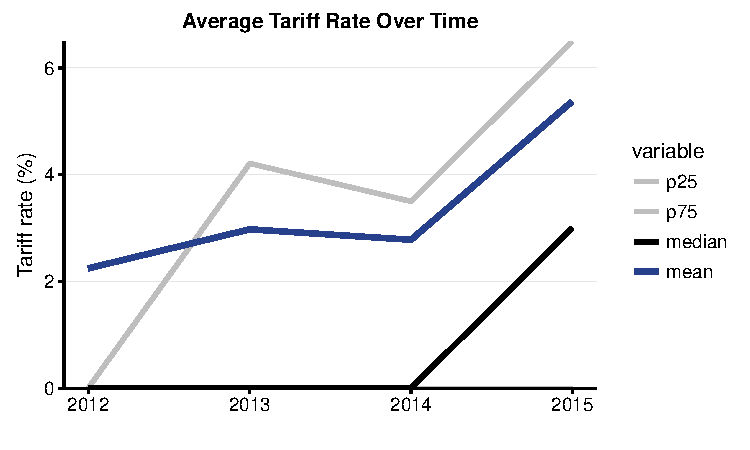
\includegraphics{Figs/tariff_summary-1} \end{center}

\begin{Shaded}
\begin{Highlighting}[]
\CommentTok{#Across products?}
\NormalTok{products <-}\StringTok{ }\NormalTok{hs12_all_tariffs[, .(}\DataTypeTok{mean =} \KeywordTok{as.double}\NormalTok{(}\KeywordTok{mean}\NormalTok{(SimpleAverage)),}
                                 \DataTypeTok{median =} \KeywordTok{as.double}\NormalTok{(}\KeywordTok{median}\NormalTok{(SimpleAverage)),}
                                 \DataTypeTok{p25 =} \KeywordTok{as.double}\NormalTok{(}\KeywordTok{quantile}\NormalTok{(SimpleAverage,.}\DecValTok{25}\NormalTok{)),}
                                 \DataTypeTok{p75 =} \KeywordTok{as.double}\NormalTok{(}\KeywordTok{quantile}\NormalTok{(SimpleAverage,.}\DecValTok{75}\NormalTok{))}
\NormalTok{),}
\NormalTok{by=}\StringTok{ }\NormalTok{ProductCode]}

\KeywordTok{ggplot}\NormalTok{(}\DataTypeTok{data=}\NormalTok{products, }\KeywordTok{aes}\NormalTok{(mean)) +}
\StringTok{  }\KeywordTok{geom_histogram}\NormalTok{(}\DataTypeTok{col=}\StringTok{"royalblue4"}\NormalTok{,}
                 \DataTypeTok{fill=}\StringTok{"royalblue4"}\NormalTok{,}
                 \DataTypeTok{alpha=}\NormalTok{.}\DecValTok{2}\NormalTok{) +}
\StringTok{  }\KeywordTok{background_grid}\NormalTok{(}\DataTypeTok{major =} \StringTok{'y'}\NormalTok{, }\DataTypeTok{minor =} \StringTok{"none"}\NormalTok{) +}
\StringTok{  }\KeywordTok{scale_y_continuous}\NormalTok{(}\DataTypeTok{expand =} \KeywordTok{c}\NormalTok{(}\DecValTok{0}\NormalTok{, }\DecValTok{0}\NormalTok{), }\DataTypeTok{limits =} \KeywordTok{c}\NormalTok{(}\DecValTok{0}\NormalTok{,}\DecValTok{3000}\NormalTok{))  +}
\StringTok{  }\KeywordTok{labs}\NormalTok{(}\DataTypeTok{title=}\StringTok{"Mean Tariff Rate Across Products"}\NormalTok{) +}
\StringTok{  }\KeywordTok{labs}\NormalTok{(}\DataTypeTok{x=}\StringTok{"Tariff rate (%)"}\NormalTok{, }\DataTypeTok{y=}\StringTok{"Number of products"}\NormalTok{)}
\end{Highlighting}
\end{Shaded}

\begin{center}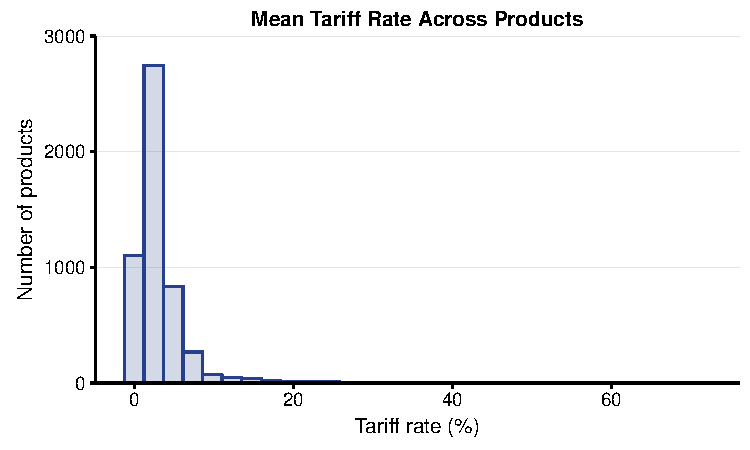
\includegraphics{Figs/tariff_summary-2} \end{center}

\begin{Shaded}
\begin{Highlighting}[]
\KeywordTok{ggplot}\NormalTok{(}\DataTypeTok{data=}\NormalTok{products, }\KeywordTok{aes}\NormalTok{(median)) +}
\StringTok{  }\KeywordTok{geom_histogram}\NormalTok{(}\DataTypeTok{col=}\StringTok{"royalblue4"}\NormalTok{,}
                 \DataTypeTok{fill=}\StringTok{"royalblue4"}\NormalTok{,}
                 \DataTypeTok{alpha=}\NormalTok{.}\DecValTok{2}\NormalTok{) +}
\StringTok{  }\KeywordTok{background_grid}\NormalTok{(}\DataTypeTok{major =} \StringTok{'y'}\NormalTok{, }\DataTypeTok{minor =} \StringTok{"none"}\NormalTok{) +}
\StringTok{  }\KeywordTok{scale_y_continuous}\NormalTok{(}\DataTypeTok{expand =} \KeywordTok{c}\NormalTok{(}\DecValTok{0}\NormalTok{, }\DecValTok{0}\NormalTok{), }\DataTypeTok{limits =} \KeywordTok{c}\NormalTok{(}\DecValTok{0}\NormalTok{, }\DecValTok{5000}\NormalTok{)) +}
\StringTok{  }\KeywordTok{labs}\NormalTok{(}\DataTypeTok{title=}\StringTok{"Median Tariff Rate Across Products"}\NormalTok{) +}
\StringTok{  }\KeywordTok{labs}\NormalTok{(}\DataTypeTok{x=}\StringTok{"Tariff rate (%)"}\NormalTok{, }\DataTypeTok{y=}\StringTok{"Number of products"}\NormalTok{)}
\end{Highlighting}
\end{Shaded}

\begin{center}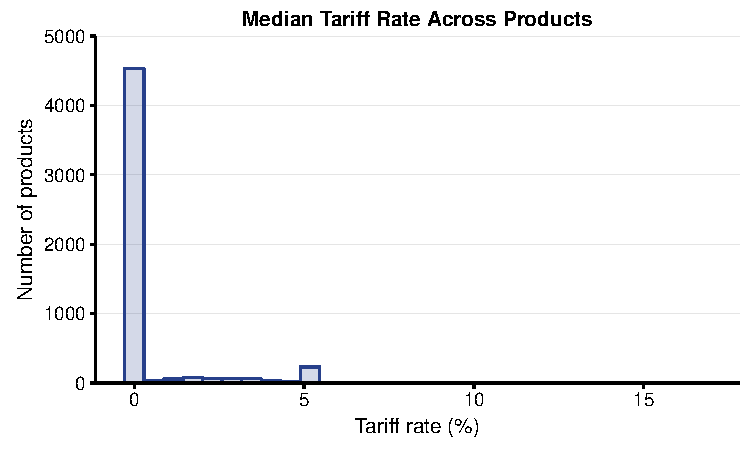
\includegraphics{Figs/tariff_summary-3} \end{center}

\begin{Shaded}
\begin{Highlighting}[]
\KeywordTok{ggplot}\NormalTok{(}\DataTypeTok{data=}\NormalTok{products, }\KeywordTok{aes}\NormalTok{(p25)) +}
\StringTok{  }\KeywordTok{geom_histogram}\NormalTok{(}\DataTypeTok{col=}\StringTok{"royalblue4"}\NormalTok{,}
                 \DataTypeTok{fill=}\StringTok{"royalblue4"}\NormalTok{,}
                 \DataTypeTok{alpha=}\NormalTok{.}\DecValTok{2}\NormalTok{) +}
\StringTok{  }\KeywordTok{background_grid}\NormalTok{(}\DataTypeTok{major =} \StringTok{'y'}\NormalTok{, }\DataTypeTok{minor =} \StringTok{"none"}\NormalTok{) +}
\StringTok{  }\KeywordTok{scale_y_continuous}\NormalTok{(}\DataTypeTok{expand =} \KeywordTok{c}\NormalTok{(}\DecValTok{0}\NormalTok{, }\DecValTok{0}\NormalTok{), }\DataTypeTok{limits =} \KeywordTok{c}\NormalTok{(}\DecValTok{0}\NormalTok{, }\DecValTok{6000}\NormalTok{), }\DataTypeTok{minor_breaks =} \OtherTok{NULL}\NormalTok{) +}
\StringTok{  }\KeywordTok{labs}\NormalTok{(}\DataTypeTok{title=}\StringTok{"25th Percentile Tariff Rate Across Products"}\NormalTok{) +}
\StringTok{  }\KeywordTok{labs}\NormalTok{(}\DataTypeTok{x=}\StringTok{"Tariff rate (%)"}\NormalTok{, }\DataTypeTok{y=}\StringTok{"Number of products"}\NormalTok{)}
\end{Highlighting}
\end{Shaded}

\begin{center}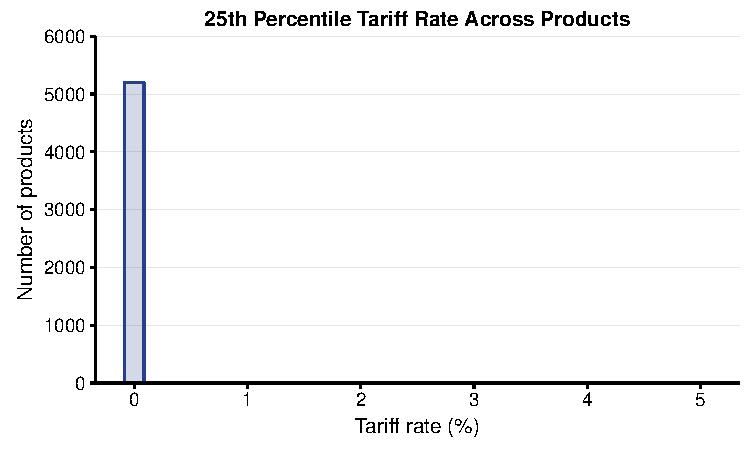
\includegraphics{Figs/tariff_summary-4} \end{center}

\begin{Shaded}
\begin{Highlighting}[]
\KeywordTok{ggplot}\NormalTok{(}\DataTypeTok{data=}\NormalTok{products, }\KeywordTok{aes}\NormalTok{(p75)) +}
\StringTok{  }\KeywordTok{geom_histogram}\NormalTok{(}\DataTypeTok{col=}\StringTok{"royalblue4"}\NormalTok{,}
                 \DataTypeTok{fill=}\StringTok{"royalblue4"}\NormalTok{,}
                 \DataTypeTok{alpha=}\NormalTok{.}\DecValTok{2}\NormalTok{) +}
\StringTok{  }\KeywordTok{background_grid}\NormalTok{(}\DataTypeTok{major =} \StringTok{'y'}\NormalTok{, }\DataTypeTok{minor =} \StringTok{"none"}\NormalTok{) +}
\StringTok{  }\KeywordTok{scale_y_continuous}\NormalTok{(}\DataTypeTok{expand =} \KeywordTok{c}\NormalTok{(}\DecValTok{0}\NormalTok{, }\DecValTok{0}\NormalTok{), }\DataTypeTok{limits =} \KeywordTok{c}\NormalTok{(}\DecValTok{0}\NormalTok{, }\DecValTok{3000}\NormalTok{),  }\DataTypeTok{minor_breaks =} \OtherTok{NULL}\NormalTok{) +}
\StringTok{  }\KeywordTok{labs}\NormalTok{(}\DataTypeTok{title=}\StringTok{"75th Percentile Tariff Rate Across Products"}\NormalTok{) +}
\StringTok{  }\KeywordTok{labs}\NormalTok{(}\DataTypeTok{x=}\StringTok{"Tariff rate (%)"}\NormalTok{, }\DataTypeTok{y=}\StringTok{"Number of products"}\NormalTok{)}
\end{Highlighting}
\end{Shaded}

\begin{center}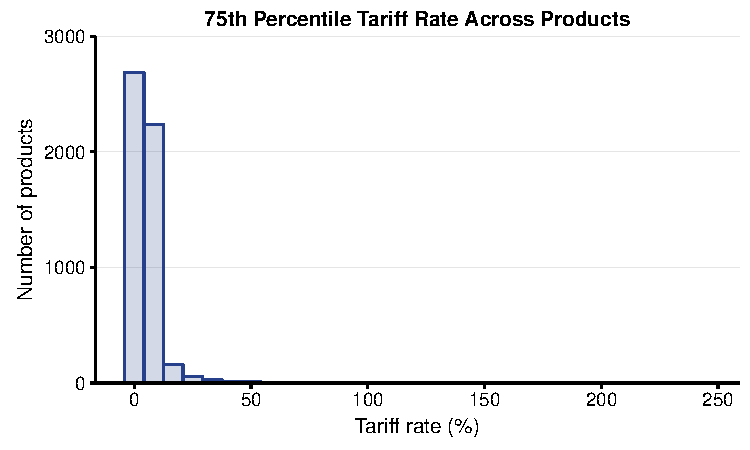
\includegraphics{Figs/tariff_summary-5} \end{center}

\begin{Shaded}
\begin{Highlighting}[]
\CommentTok{#Across countries?}
\NormalTok{countries <-}\StringTok{ }\NormalTok{hs12_all_tariffs[, .(}\DataTypeTok{mean =} \KeywordTok{as.double}\NormalTok{(}\KeywordTok{mean}\NormalTok{(SimpleAverage)),}
                                  \DataTypeTok{median =} \KeywordTok{as.double}\NormalTok{(}\KeywordTok{median}\NormalTok{(SimpleAverage)),}
                                  \DataTypeTok{p25 =} \KeywordTok{as.double}\NormalTok{(}\KeywordTok{quantile}\NormalTok{(SimpleAverage,.}\DecValTok{25}\NormalTok{)),}
                                  \DataTypeTok{p75 =} \KeywordTok{as.double}\NormalTok{(}\KeywordTok{quantile}\NormalTok{(SimpleAverage,.}\DecValTok{75}\NormalTok{))}
\NormalTok{),}
\NormalTok{by=}\StringTok{ }\KeywordTok{c}\NormalTok{(}\StringTok{"Importer"}\NormalTok{, }\StringTok{"Exporter"}\NormalTok{)]}

\KeywordTok{ggplot}\NormalTok{(}\DataTypeTok{data=}\NormalTok{countries, }\KeywordTok{aes}\NormalTok{(mean)) +}
\StringTok{  }\KeywordTok{geom_histogram}\NormalTok{(}\DataTypeTok{col=}\StringTok{"royalblue4"}\NormalTok{,}
                 \DataTypeTok{fill=}\StringTok{"royalblue4"}\NormalTok{,}
                 \DataTypeTok{alpha=}\NormalTok{.}\DecValTok{2}\NormalTok{) +}
\StringTok{  }\KeywordTok{background_grid}\NormalTok{(}\DataTypeTok{major =} \StringTok{'y'}\NormalTok{, }\DataTypeTok{minor =} \StringTok{"none"}\NormalTok{) +}
\StringTok{  }\KeywordTok{scale_y_continuous}\NormalTok{(}\DataTypeTok{expand =} \KeywordTok{c}\NormalTok{(}\DecValTok{0}\NormalTok{, }\DecValTok{0}\NormalTok{), }\DataTypeTok{limits =} \KeywordTok{c}\NormalTok{(}\DecValTok{0}\NormalTok{, }\DecValTok{10000}\NormalTok{), }\DataTypeTok{minor_breaks =} \OtherTok{NULL}\NormalTok{) +}
\StringTok{  }\KeywordTok{labs}\NormalTok{(}\DataTypeTok{title=}\StringTok{"Mean Tariff Rate Across Country Pairs"}\NormalTok{) +}
\StringTok{  }\KeywordTok{labs}\NormalTok{(}\DataTypeTok{x=}\StringTok{"Tariff Rate (%)"}\NormalTok{, }\DataTypeTok{y=}\StringTok{"Number of pairs"}\NormalTok{)}
\end{Highlighting}
\end{Shaded}

\begin{center}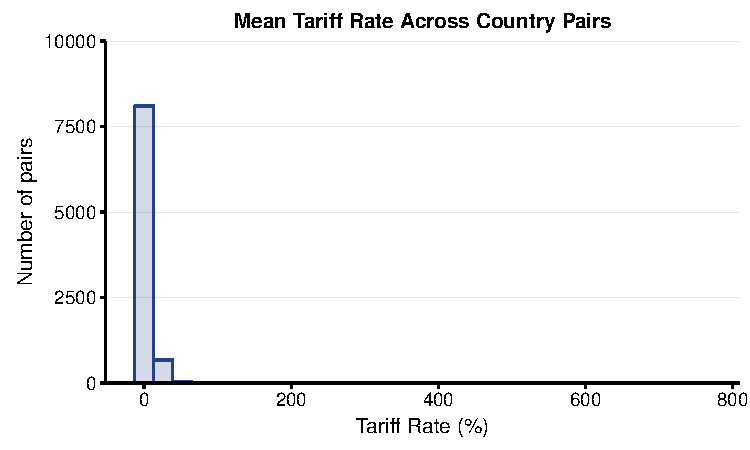
\includegraphics{Figs/tariff_summary-6} \end{center}

\begin{Shaded}
\begin{Highlighting}[]
\KeywordTok{ggplot}\NormalTok{(}\DataTypeTok{data=}\NormalTok{countries, }\KeywordTok{aes}\NormalTok{(median)) +}
\StringTok{  }\KeywordTok{geom_histogram}\NormalTok{(}\DataTypeTok{col=}\StringTok{"royalblue4"}\NormalTok{,}
                 \DataTypeTok{fill=}\StringTok{"royalblue4"}\NormalTok{,}
                 \DataTypeTok{alpha=}\NormalTok{.}\DecValTok{2}\NormalTok{) +}
\StringTok{  }\KeywordTok{background_grid}\NormalTok{(}\DataTypeTok{major =} \StringTok{'y'}\NormalTok{, }\DataTypeTok{minor =} \StringTok{"none"}\NormalTok{) +}
\StringTok{  }\KeywordTok{scale_y_continuous}\NormalTok{(}\DataTypeTok{expand =} \KeywordTok{c}\NormalTok{(}\DecValTok{0}\NormalTok{, }\DecValTok{0}\NormalTok{), }\DataTypeTok{limits =} \KeywordTok{c}\NormalTok{(}\DecValTok{0}\NormalTok{, }\DecValTok{10000}\NormalTok{), }\DataTypeTok{minor_breaks =} \OtherTok{NULL}\NormalTok{) +}
\StringTok{  }\KeywordTok{labs}\NormalTok{(}\DataTypeTok{title=}\StringTok{"Median Tariff Rate Across Country Pairs"}\NormalTok{) +}
\StringTok{  }\KeywordTok{labs}\NormalTok{(}\DataTypeTok{x=}\StringTok{"Tariff Rate (%)"}\NormalTok{, }\DataTypeTok{y=}\StringTok{"Number of pairs"}\NormalTok{)}
\end{Highlighting}
\end{Shaded}

\begin{center}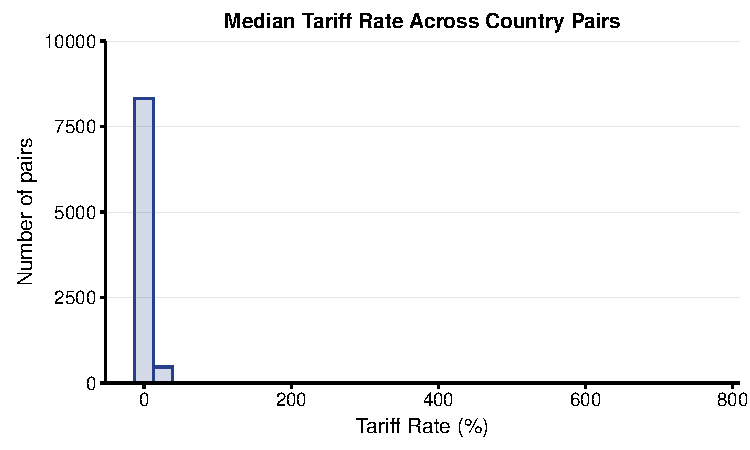
\includegraphics{Figs/tariff_summary-7} \end{center}

\begin{Shaded}
\begin{Highlighting}[]
\KeywordTok{ggplot}\NormalTok{(}\DataTypeTok{data=}\NormalTok{countries, }\KeywordTok{aes}\NormalTok{(p25)) +}
\StringTok{  }\KeywordTok{geom_histogram}\NormalTok{(}\DataTypeTok{col=}\StringTok{"royalblue4"}\NormalTok{,}
                 \DataTypeTok{fill=}\StringTok{"royalblue4"}\NormalTok{,}
                 \DataTypeTok{alpha=}\NormalTok{.}\DecValTok{2}\NormalTok{) +}
\StringTok{  }\KeywordTok{background_grid}\NormalTok{(}\DataTypeTok{major =} \StringTok{'y'}\NormalTok{, }\DataTypeTok{minor =} \StringTok{"none"}\NormalTok{) +}
\StringTok{  }\KeywordTok{scale_y_continuous}\NormalTok{(}\DataTypeTok{expand =} \KeywordTok{c}\NormalTok{(}\DecValTok{0}\NormalTok{, }\DecValTok{0}\NormalTok{), }\DataTypeTok{limits =} \KeywordTok{c}\NormalTok{(}\DecValTok{0}\NormalTok{, }\DecValTok{10000}\NormalTok{), }\DataTypeTok{minor_breaks =} \OtherTok{NULL}\NormalTok{) +}
\StringTok{  }\KeywordTok{labs}\NormalTok{(}\DataTypeTok{title=}\StringTok{"25th Percentile Tariff Rate Across Country Pairs"}\NormalTok{) +}
\StringTok{  }\KeywordTok{labs}\NormalTok{(}\DataTypeTok{x=}\StringTok{"Tariff Rate (%)"}\NormalTok{, }\DataTypeTok{y=}\StringTok{"Number of pairs"}\NormalTok{)}
\end{Highlighting}
\end{Shaded}

\begin{center}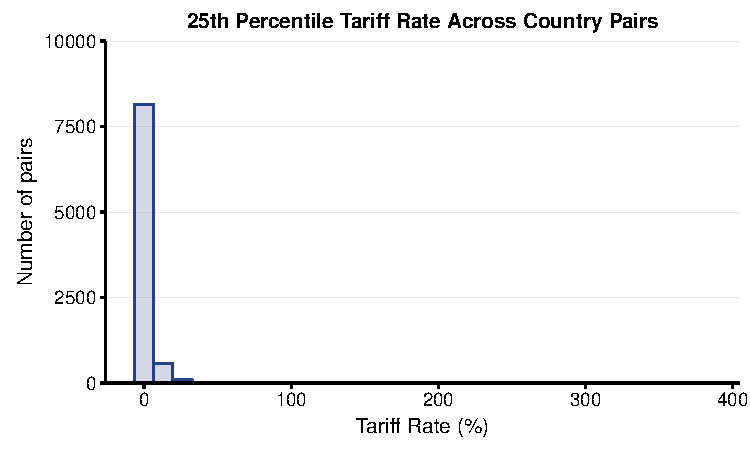
\includegraphics{Figs/tariff_summary-8} \end{center}

\begin{Shaded}
\begin{Highlighting}[]
\KeywordTok{ggplot}\NormalTok{(}\DataTypeTok{data=}\NormalTok{countries, }\KeywordTok{aes}\NormalTok{(p75)) +}
\StringTok{  }\KeywordTok{geom_histogram}\NormalTok{(}\DataTypeTok{col=}\StringTok{"royalblue4"}\NormalTok{,}
                 \DataTypeTok{fill=}\StringTok{"royalblue4"}\NormalTok{,}
                 \DataTypeTok{alpha=}\NormalTok{.}\DecValTok{2}\NormalTok{) +}
\StringTok{  }\KeywordTok{background_grid}\NormalTok{(}\DataTypeTok{major =} \StringTok{'y'}\NormalTok{, }\DataTypeTok{minor =} \StringTok{"none"}\NormalTok{) +}
\StringTok{  }\KeywordTok{scale_y_continuous}\NormalTok{(}\DataTypeTok{expand =} \KeywordTok{c}\NormalTok{(}\DecValTok{0}\NormalTok{, }\DecValTok{0}\NormalTok{), }\DataTypeTok{limits =} \KeywordTok{c}\NormalTok{(}\DecValTok{0}\NormalTok{, }\DecValTok{10000}\NormalTok{), }\DataTypeTok{minor_breaks =} \OtherTok{NULL}\NormalTok{) +}
\StringTok{  }\KeywordTok{labs}\NormalTok{(}\DataTypeTok{title=}\StringTok{"75th Percentile Tariff Rate Across Country Pairs"}\NormalTok{) +}
\StringTok{  }\KeywordTok{labs}\NormalTok{(}\DataTypeTok{x=}\StringTok{"Tariff Rate (%)"}\NormalTok{, }\DataTypeTok{y=}\StringTok{"Number of pairs"}\NormalTok{)}
\end{Highlighting}
\end{Shaded}

\begin{center}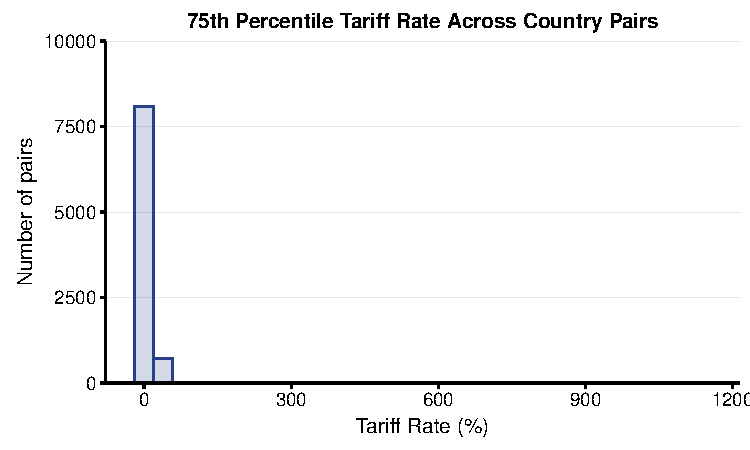
\includegraphics{Figs/tariff_summary-9} \end{center}

\begin{Shaded}
\begin{Highlighting}[]
\KeywordTok{rm}\NormalTok{(Years, products, countries, hs12_all_tariffs)}

\CommentTok{#Regress trade gap on dummies and plot coefficients }

\KeywordTok{load}\NormalTok{(}\KeywordTok{paste}\NormalTok{(DataPath,}\StringTok{"Analysis Data/hs12_all_tariffs_qty.Rda"}\NormalTok{, }\DataTypeTok{sep =} \StringTok{"/"}\NormalTok{))}
\NormalTok{hs12_all_tariffs <-}\StringTok{ }\NormalTok{hs12_all_tariffs[!}\KeywordTok{is.na}\NormalTok{(SimpleAverage)]}

\NormalTok{hs12_all_tariffs <-}\StringTok{ }\NormalTok{hs12_all_tariffs[, }
                    \NormalTok{.(Year, ProductCode, }\StringTok{`}\DataTypeTok{Reporter_ISO_N}\StringTok{`}\NormalTok{, }\StringTok{`}\DataTypeTok{Partner Code}\StringTok{`}\NormalTok{, SimpleAverage)]}

\NormalTok{hs12_all_tariffs$Year <-}\StringTok{ }\KeywordTok{as.Date}\NormalTok{(hs12_all_tariffs$Year, }\StringTok{"%Y"}\NormalTok{)}
\NormalTok{hs12_all_tariffs$Year <-}\StringTok{ }\KeywordTok{floor_date}\NormalTok{(hs12_all_tariffs$Year,}\StringTok{"year"}\NormalTok{)}

\NormalTok{hs12_all_tariffs$Year.f <-}\StringTok{ }\KeywordTok{factor}\NormalTok{(hs12_all_tariffs$Year)}
\NormalTok{hs12_all_tariffs$Products.f <-}\StringTok{ }\KeywordTok{factor}\NormalTok{(hs12_all_tariffs$ProductCode)}

\NormalTok{hs12_all_tariffs$Importer.f <-}\StringTok{ }\KeywordTok{factor}\NormalTok{(hs12_all_tariffs$}\StringTok{`}\DataTypeTok{Reporter_ISO_N}\StringTok{`}\NormalTok{)}
\NormalTok{hs12_all_tariffs$Exporter.f <-}\StringTok{ }\KeywordTok{factor}\NormalTok{(hs12_all_tariffs$}\StringTok{`}\DataTypeTok{Partner Code}\StringTok{`}\NormalTok{)}
\NormalTok{hs12_all_tariffs$Pairs.f <-}\StringTok{ }\KeywordTok{with}\NormalTok{(hs12_all_tariffs, }\KeywordTok{interaction}\NormalTok{(Importer.f, Exporter.f))}

\NormalTok{hs12_all_tariffs <-}\StringTok{ }\NormalTok{hs12_all_tariffs[, .(Year, SimpleAverage, Year.f, Products.f, Pairs.f)]}

\NormalTok{reg <-}\StringTok{ }\KeywordTok{felm}\NormalTok{(SimpleAverage ~}\StringTok{ }\DecValTok{1} \NormalTok{|}\StringTok{ }\NormalTok{Year.f +}\StringTok{ }\NormalTok{Products.f +}\StringTok{ }\NormalTok{Pairs.f,}
            \DataTypeTok{data =} \NormalTok{hs12_all_tariffs,}
            \DataTypeTok{exactDOF =} \OtherTok{FALSE}\NormalTok{,}
            \DataTypeTok{keepX =} \OtherTok{FALSE}\NormalTok{,}
            \DataTypeTok{keepCX =} \OtherTok{FALSE}\NormalTok{)}

\NormalTok{fes <-}\StringTok{ }\KeywordTok{getfe}\NormalTok{(reg,}
             \DataTypeTok{se=}\OtherTok{TRUE}\NormalTok{,}
             \DataTypeTok{bN =} \DecValTok{50}
\NormalTok{)}

\NormalTok{Yearfes <-}\StringTok{ }\KeywordTok{subset}\NormalTok{(fes,fe ==}\StringTok{ "Year.f"}\NormalTok{)}

\NormalTok{Yearfes$ci_ub <-}\StringTok{ }\NormalTok{Yearfes$effect +}\StringTok{ }\NormalTok{(}\FloatTok{1.96} \NormalTok{*}\StringTok{ }\NormalTok{Yearfes$se)}
\NormalTok{Yearfes$ci_lb <-}\StringTok{ }\NormalTok{Yearfes$effect -}\StringTok{ }\NormalTok{(}\FloatTok{1.96} \NormalTok{*}\StringTok{ }\NormalTok{Yearfes$se)}
\NormalTok{Yearfes <-}\StringTok{ }\KeywordTok{merge}\NormalTok{(Yearfes,}\KeywordTok{unique}\NormalTok{(hs12_all_tariffs[,}\KeywordTok{list}\NormalTok{(Year,Year.f)]),}\DataTypeTok{by.x =} \StringTok{"idx"}\NormalTok{,}\DataTypeTok{by.y=}\StringTok{"Year.f"}\NormalTok{)}

\KeywordTok{ggplot}\NormalTok{(}\DataTypeTok{data =} \NormalTok{Yearfes, }\KeywordTok{aes}\NormalTok{(Year,effect)) +}
\StringTok{  }\KeywordTok{geom_errorbar}\NormalTok{(}\KeywordTok{aes}\NormalTok{(}\DataTypeTok{ymin =} \NormalTok{ci_lb, }\DataTypeTok{ymax =} \NormalTok{ci_ub), }\DataTypeTok{color =} \StringTok{"grey35"}\NormalTok{) +}
\StringTok{  }\KeywordTok{geom_line}\NormalTok{(}\DataTypeTok{color =} \StringTok{"royalblue4"}\NormalTok{, }\DataTypeTok{size =} \DecValTok{1}\NormalTok{) +}
\StringTok{  }\KeywordTok{geom_point}\NormalTok{(}\DataTypeTok{color =} \StringTok{"royalblue4"}\NormalTok{) +}
\StringTok{  }\KeywordTok{background_grid}\NormalTok{(}\DataTypeTok{major =} \StringTok{'y'}\NormalTok{, }\DataTypeTok{minor =} \StringTok{"none"}\NormalTok{) +}
\StringTok{  }\KeywordTok{scale_y_continuous}\NormalTok{(}\DataTypeTok{expand =} \KeywordTok{c}\NormalTok{(}\DecValTok{0}\NormalTok{, }\DecValTok{0}\NormalTok{), }\DataTypeTok{limits =} \KeywordTok{c}\NormalTok{(-}\DecValTok{3}\NormalTok{,}\DecValTok{1}\NormalTok{), }\DataTypeTok{minor_breaks =} \OtherTok{NULL}\NormalTok{) +}
\StringTok{  }\KeywordTok{xlab}\NormalTok{(}\DataTypeTok{label =} \StringTok{""}\NormalTok{) +}
\StringTok{  }\KeywordTok{ylab}\NormalTok{(}\DataTypeTok{label =} \StringTok{"Tariff rate (%)"}\NormalTok{) +}
\StringTok{  }\KeywordTok{labs}\NormalTok{(}\DataTypeTok{title =} \StringTok{"Tariff Rate Over Time, Controlling for Product/Country Pairs"}\NormalTok{)}
\end{Highlighting}
\end{Shaded}

\begin{center}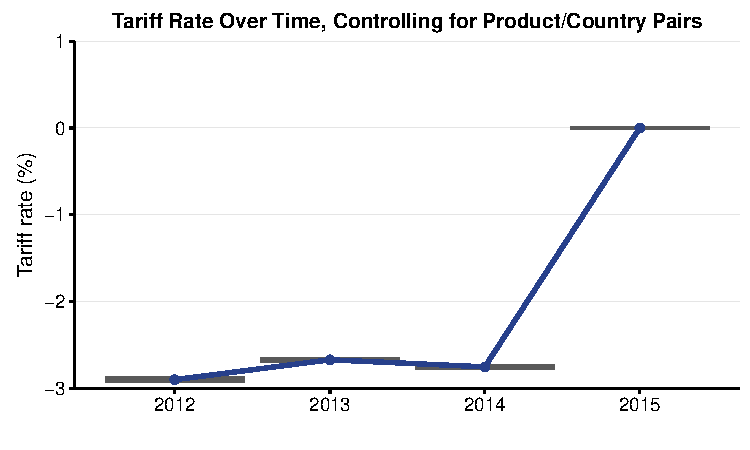
\includegraphics{Figs/tariff_summary-10} \end{center}

\begin{Shaded}
\begin{Highlighting}[]
\NormalTok{productfes <-}\StringTok{ }\KeywordTok{subset}\NormalTok{(fes,fe ==}\StringTok{ "Products.f"}\NormalTok{)}
\NormalTok{productfes <-}\StringTok{ }\NormalTok{productfes[,}\KeywordTok{c}\NormalTok{(}\StringTok{"effect"}\NormalTok{,}\StringTok{"idx"}\NormalTok{)]}

\KeywordTok{ggplot}\NormalTok{(}\DataTypeTok{data=}\NormalTok{productfes, }\KeywordTok{aes}\NormalTok{(effect)) +}
\StringTok{  }\KeywordTok{geom_histogram}\NormalTok{(}\DataTypeTok{col=}\StringTok{"royalblue4"}\NormalTok{,}
                 \DataTypeTok{fill=}\StringTok{"royalblue4"}\NormalTok{,}
                 \DataTypeTok{alpha=}\NormalTok{.}\DecValTok{2}\NormalTok{) +}
\StringTok{  }\KeywordTok{background_grid}\NormalTok{(}\DataTypeTok{major =} \StringTok{'y'}\NormalTok{, }\DataTypeTok{minor =} \StringTok{"none"}\NormalTok{) +}
\StringTok{  }\KeywordTok{scale_y_continuous}\NormalTok{(}\DataTypeTok{expand =} \KeywordTok{c}\NormalTok{(}\DecValTok{0}\NormalTok{, }\DecValTok{0}\NormalTok{), }\DataTypeTok{limits =} \KeywordTok{c}\NormalTok{(}\DecValTok{0}\NormalTok{,}\DecValTok{3000}\NormalTok{), }\DataTypeTok{minor_breaks =} \OtherTok{NULL}\NormalTok{) +}
\StringTok{  }\KeywordTok{labs}\NormalTok{(}\DataTypeTok{title=}\StringTok{"Mean Tariff Rate Across Products, Controlling for Country Pairs/Years"}\NormalTok{) +}
\StringTok{  }\KeywordTok{labs}\NormalTok{(}\DataTypeTok{x=}\StringTok{"Tariff rate (%)"}\NormalTok{, }\DataTypeTok{y=}\StringTok{"Number of products"}\NormalTok{)}
\end{Highlighting}
\end{Shaded}

\begin{center}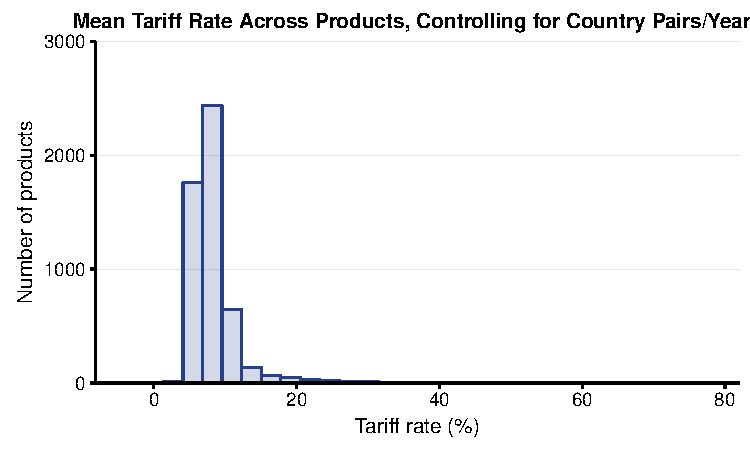
\includegraphics{Figs/tariff_summary-11} \end{center}

\begin{Shaded}
\begin{Highlighting}[]
\NormalTok{pairfes <-}\StringTok{ }\KeywordTok{subset}\NormalTok{(fes,fe ==}\StringTok{ "Pairs.f"}\NormalTok{)}
\NormalTok{pairfes <-}\StringTok{ }\NormalTok{pairfes[,}\KeywordTok{c}\NormalTok{(}\StringTok{"effect"}\NormalTok{,}\StringTok{"idx"}\NormalTok{)]}

\KeywordTok{ggplot}\NormalTok{(}\DataTypeTok{data=}\NormalTok{pairfes, }\KeywordTok{aes}\NormalTok{(effect)) +}
\StringTok{  }\KeywordTok{geom_histogram}\NormalTok{(}\DataTypeTok{col=}\StringTok{"royalblue4"}\NormalTok{,}
                 \DataTypeTok{fill=}\StringTok{"royalblue4"}\NormalTok{,}
                 \DataTypeTok{alpha=}\NormalTok{.}\DecValTok{2}\NormalTok{) +}
\StringTok{  }\KeywordTok{background_grid}\NormalTok{(}\DataTypeTok{major =} \StringTok{'y'}\NormalTok{, }\DataTypeTok{minor =} \StringTok{"none"}\NormalTok{) +}
\StringTok{  }\KeywordTok{scale_y_continuous}\NormalTok{(}\DataTypeTok{expand =} \KeywordTok{c}\NormalTok{(}\DecValTok{0}\NormalTok{, }\DecValTok{0}\NormalTok{), }\DataTypeTok{limits =} \KeywordTok{c}\NormalTok{(}\DecValTok{0}\NormalTok{, }\DecValTok{10000}\NormalTok{), }\DataTypeTok{minor_breaks =} \OtherTok{NULL}\NormalTok{) +}
\StringTok{  }\KeywordTok{labs}\NormalTok{(}\DataTypeTok{title=}\StringTok{"Mean Tariff Rate Across Country Pairs, Controlling for Products/Years"}\NormalTok{) +}
\StringTok{  }\KeywordTok{labs}\NormalTok{(}\DataTypeTok{x=}\StringTok{"Tariff rate (%)"}\NormalTok{, }\DataTypeTok{y=}\StringTok{"Number of country pairs"}\NormalTok{)}
\end{Highlighting}
\end{Shaded}

\begin{center}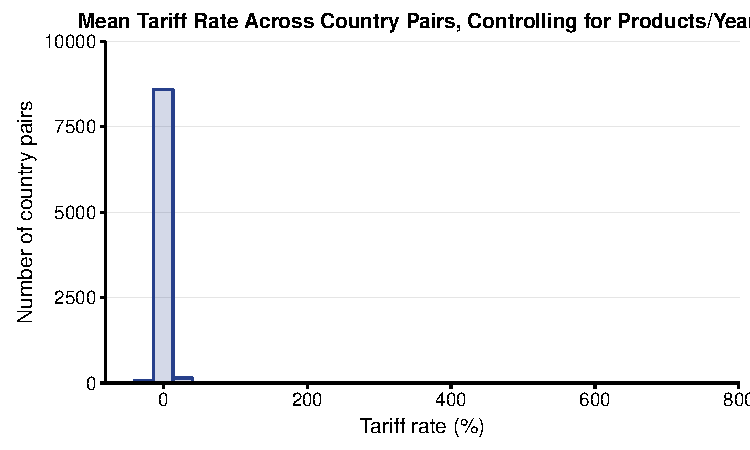
\includegraphics{Figs/tariff_summary-12} \end{center}

\begin{Shaded}
\begin{Highlighting}[]
\KeywordTok{rm}\NormalTok{(fes, hs12_all_tariffs, pairfes, Yearfes, productfes, reg)}
\end{Highlighting}
\end{Shaded}

\section{Tariff vs.~Trade Data, Quantity
Gap}\label{tariff-vs.trade-data-quantity-gap}

The following figure plots the quantity evasion gap against mean
``Simple Average'' tariff rates, grouped by each tariff rate that
appears in the data.

\begin{Shaded}
\begin{Highlighting}[]
\KeywordTok{load}\NormalTok{(}\KeywordTok{paste}\NormalTok{(DataPath,}\StringTok{"Analysis Data/hs12_all_tariffs_qty.Rda"}\NormalTok{, }\DataTypeTok{sep =} \StringTok{"/"}\NormalTok{))}

\NormalTok{hs12_all_tariffs <-}\StringTok{ }\NormalTok{hs12_all_tariffs[, }
                    \NormalTok{.(Year, ProductCode, Importer, Exporter, SimpleAverage, Qty_log_gap)]}

\NormalTok{hs12_all_tariffs <-}\StringTok{ }\NormalTok{hs12_all_tariffs[!}\KeywordTok{is.na}\NormalTok{(SimpleAverage)]}

\NormalTok{tariffs <-}\StringTok{ }\NormalTok{hs12_all_tariffs[, .(}\DataTypeTok{mean =} \KeywordTok{mean}\NormalTok{(Qty_log_gap)), by =}\StringTok{ }\NormalTok{SimpleAverage]}

\NormalTok{tariffs <-}\StringTok{ }\KeywordTok{melt}\NormalTok{(tariffs, }\DataTypeTok{id =} \StringTok{"SimpleAverage"}\NormalTok{)}
\NormalTok{tariffs <-}\StringTok{ }\KeywordTok{rename}\NormalTok{(tariffs, }\StringTok{"Legend"} \NormalTok{=}\StringTok{ "variable"}\NormalTok{) }

\KeywordTok{ggplot}\NormalTok{(tariffs, }\KeywordTok{aes}\NormalTok{(SimpleAverage, value, }\DataTypeTok{colour=}\NormalTok{Legend)) +}
\StringTok{  }\KeywordTok{geom_point}\NormalTok{(}\KeywordTok{aes}\NormalTok{(}\DataTypeTok{colour =} \NormalTok{Legend), }\DataTypeTok{size =} \DecValTok{2}\NormalTok{, }\DataTypeTok{alpha =} \NormalTok{.}\DecValTok{2}\NormalTok{) +}
\StringTok{  }\KeywordTok{geom_smooth}\NormalTok{(}\DataTypeTok{method =} \StringTok{"lm"}\NormalTok{) +}
\StringTok{  }\KeywordTok{scale_colour_manual}\NormalTok{(}\DataTypeTok{values=}\KeywordTok{c}\NormalTok{(}\StringTok{"royalblue4"}\NormalTok{)) +}
\StringTok{  }\KeywordTok{labs}\NormalTok{(}\DataTypeTok{title=}\StringTok{"Quantity Gap at Different Tariff Rates, 2012-2015"}\NormalTok{) +}
\StringTok{  }\KeywordTok{background_grid}\NormalTok{(}\DataTypeTok{major =} \StringTok{'y'}\NormalTok{, }\DataTypeTok{minor =} \StringTok{"none"}\NormalTok{) +}
\StringTok{  }\KeywordTok{labs}\NormalTok{(}\DataTypeTok{x=}\StringTok{"Tariff rate (%)"}\NormalTok{, }\DataTypeTok{y=}\StringTok{"Quantity gap, log scale"}\NormalTok{) +}
\StringTok{  }\KeywordTok{labs}\NormalTok{(}\DataTypeTok{caption=}\StringTok{"Each point represents a unique tariff rate"}\NormalTok{) +}
\StringTok{  }\KeywordTok{theme}\NormalTok{(}\DataTypeTok{legend.position=}\StringTok{"none"}\NormalTok{)}
\end{Highlighting}
\end{Shaded}

\begin{center}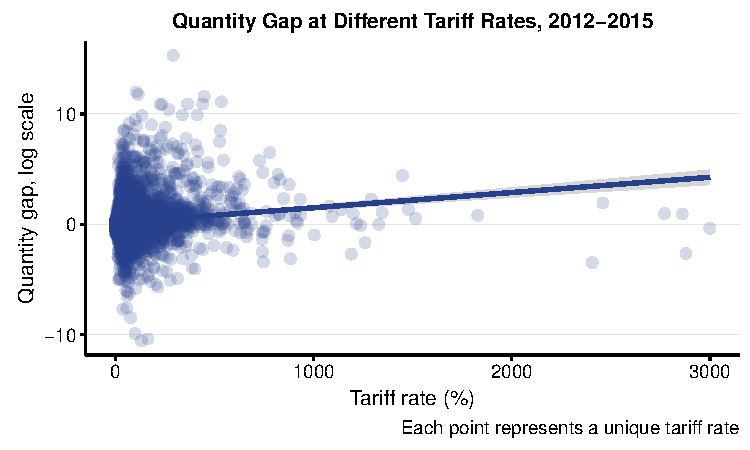
\includegraphics{Figs/tariffVtrade_fig1-1} \end{center}

The next figure repeats the first, but with tariff rates grouped to the
nearest round number and zoomed in to tariff rates between 0 and 300\%.

\begin{Shaded}
\begin{Highlighting}[]
\NormalTok{tariffs <-}\StringTok{ }\NormalTok{hs12_all_tariffs[SimpleAverage <=}\StringTok{ }\DecValTok{300}\NormalTok{, ]}
\NormalTok{tariffs$SimpleAverage <-}\StringTok{ }\KeywordTok{round}\NormalTok{(tariffs$SimpleAverage, }\DataTypeTok{digits =} \DecValTok{0}\NormalTok{)}

\NormalTok{tariffs <-}\StringTok{ }\NormalTok{tariffs[, .(}\DataTypeTok{mean =} \KeywordTok{mean}\NormalTok{(Qty_log_gap)), by =}\StringTok{ }\NormalTok{SimpleAverage]}

\NormalTok{tariffs <-}\StringTok{ }\KeywordTok{melt}\NormalTok{(tariffs, }\DataTypeTok{id =} \StringTok{"SimpleAverage"}\NormalTok{)}
\NormalTok{tariffs <-}\StringTok{ }\KeywordTok{rename}\NormalTok{(tariffs, }\StringTok{"Legend"} \NormalTok{=}\StringTok{ "variable"}\NormalTok{) }

\KeywordTok{ggplot}\NormalTok{(tariffs, }\KeywordTok{aes}\NormalTok{(SimpleAverage, value, }\DataTypeTok{colour=}\NormalTok{Legend)) +}
\StringTok{  }\KeywordTok{geom_point}\NormalTok{(}\KeywordTok{aes}\NormalTok{(}\DataTypeTok{colour =} \NormalTok{Legend), }\DataTypeTok{size =} \DecValTok{2}\NormalTok{, }\DataTypeTok{alpha =} \NormalTok{.}\DecValTok{2}\NormalTok{) +}
\StringTok{  }\KeywordTok{geom_smooth}\NormalTok{(}\DataTypeTok{method =} \StringTok{"lm"}\NormalTok{) +}
\StringTok{  }\KeywordTok{scale_colour_manual}\NormalTok{(}\DataTypeTok{values=}\KeywordTok{c}\NormalTok{(}\StringTok{"royalblue4"}\NormalTok{)) +}
\StringTok{  }\KeywordTok{labs}\NormalTok{(}\DataTypeTok{title=}\StringTok{"Quantity Gap at Different Tariff Rates, 2012-2015"}\NormalTok{) +}
\StringTok{  }\KeywordTok{scale_y_continuous}\NormalTok{(}\DataTypeTok{expand =} \KeywordTok{c}\NormalTok{(}\DecValTok{0}\NormalTok{, }\DecValTok{0}\NormalTok{), }\DataTypeTok{limits =} \KeywordTok{c}\NormalTok{(-}\DecValTok{5}\NormalTok{, }\DecValTok{5}\NormalTok{)) +}
\StringTok{  }\KeywordTok{background_grid}\NormalTok{(}\DataTypeTok{major =} \StringTok{'y'}\NormalTok{, }\DataTypeTok{minor =} \StringTok{"none"}\NormalTok{) +}
\StringTok{  }\KeywordTok{labs}\NormalTok{(}\DataTypeTok{x=}\StringTok{"Tariff rate (%)"}\NormalTok{, }\DataTypeTok{y=}\StringTok{"Quantity gap, log scale"}\NormalTok{) +}
\StringTok{  }\KeywordTok{labs}\NormalTok{(}\DataTypeTok{caption=}\StringTok{"Each point = average tariff rate, rounded to nearest whole number"}\NormalTok{) +}\StringTok{ }
\StringTok{  }\KeywordTok{theme}\NormalTok{(}\DataTypeTok{legend.position=}\StringTok{"none"}\NormalTok{)}
\end{Highlighting}
\end{Shaded}

\begin{verbatim}
## Warning: Removed 2 rows containing non-finite values (stat_smooth).
\end{verbatim}

\begin{verbatim}
## Warning: Removed 2 rows containing missing values (geom_point).
\end{verbatim}

\begin{center}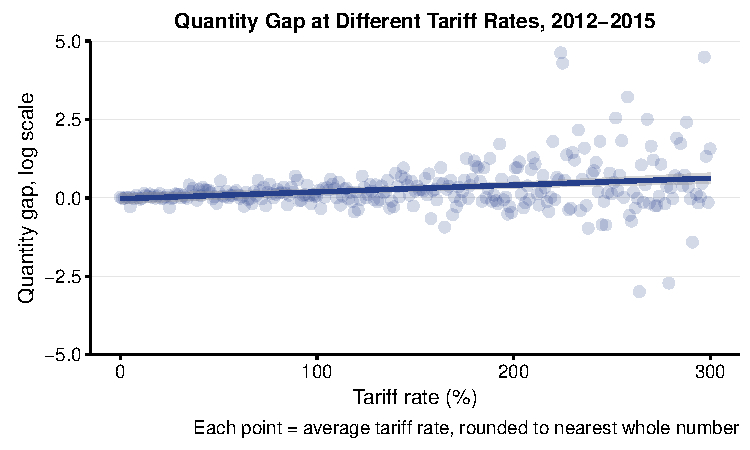
\includegraphics{Figs/tariffVtrade_fig2-1} \end{center}

Next, a simple regression of the quantity evasion gap regressed on the
simple average tariff rate:

\begin{Shaded}
\begin{Highlighting}[]
\NormalTok{simpreg =}\StringTok{ }\KeywordTok{lm}\NormalTok{(Qty_log_gap ~}\StringTok{ }\NormalTok{SimpleAverage, }\DataTypeTok{data =} \NormalTok{hs12_all_tariffs)}
\KeywordTok{summary}\NormalTok{(simpreg)}
\end{Highlighting}
\end{Shaded}

\begin{verbatim}
## 
## Call:
## lm(formula = Qty_log_gap ~ SimpleAverage, data = hs12_all_tariffs)
## 
## Residuals:
##      Min       1Q   Median       3Q      Max 
## -21.3690  -1.0005   0.0058   1.0323  19.5888 
## 
## Coefficients:
##                 Estimate Std. Error t value Pr(>|t|)    
## (Intercept)   -5.822e-03  7.464e-04    -7.8 6.19e-15 ***
## SimpleAverage  6.308e-04  5.898e-05    10.7  < 2e-16 ***
## ---
## Signif. codes:  0 '***' 0.001 '**' 0.01 '*' 0.05 '.' 0.1 ' ' 1
## 
## Residual standard error: 2.425 on 11401271 degrees of freedom
## Multiple R-squared:  1.003e-05,  Adjusted R-squared:  9.944e-06 
## F-statistic: 114.4 on 1 and 11401271 DF,  p-value: < 2.2e-16
\end{verbatim}


\end{document}
